\chapter{Luminosity Measurement}

Once the final calibration constant of the PCC detector has been obtained using data primarily from the vdM program, the next step is to apply this calibration to the luminosity measured by the detector throughout the entire year of data acquisition. This chapter will detail the specifications of these so-called physics data and the various analyses conducted to determine the final luminosity, including the analysis of detector modules and background (afterglow) for each year. Additionally, cross-checks with other luminometers will be performed to ultimately determine the final uncertainty in the luminosity measurement.


\section{Physics Data}


In June 2017, data collection for the second phase of Run 2 of the Large Hadron Collider (LHC) began, covering the years 2017 and 2018. This period resulted in a total recorded luminosity of \(49.81 \, \text{fb}^{-1}\) for 2017 and \(67.86 \, \text{fb}^{-1}\) for 2018, collected during proton-proton collisions at a center-of-mass energy of \(\sqrt{s} = 13\) TeV.

The data-taking process started with the establishment of stable beams and continued until either the beam was intentionally stopped or temporarily interrupted for beam studies. The total luminosity delivered by the LHC to CMS (in blue) and the luminosity recorded by CMS (in orange) for 2017 and 2018 are illustrated in Figures~\ref{Lumi_2017} and~\ref{Lumi_2018}, respectively~\citep{wikicern}.

\begin{figure}[h!]
    \centering
    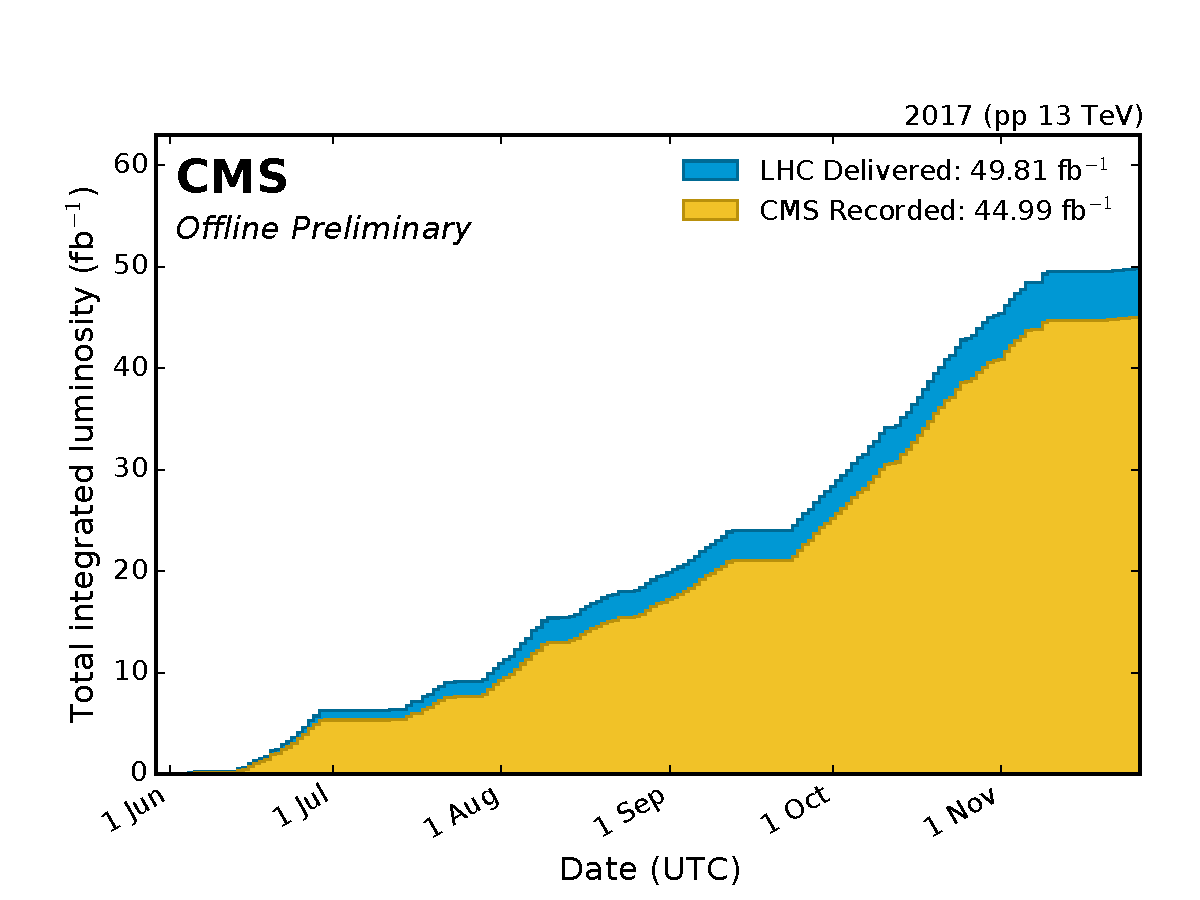
\includegraphics[width=.45\textwidth]{Chapter3/Luminosity/int_lumi_per_day_cumulative_pp_2017_Normtag.pdf}
    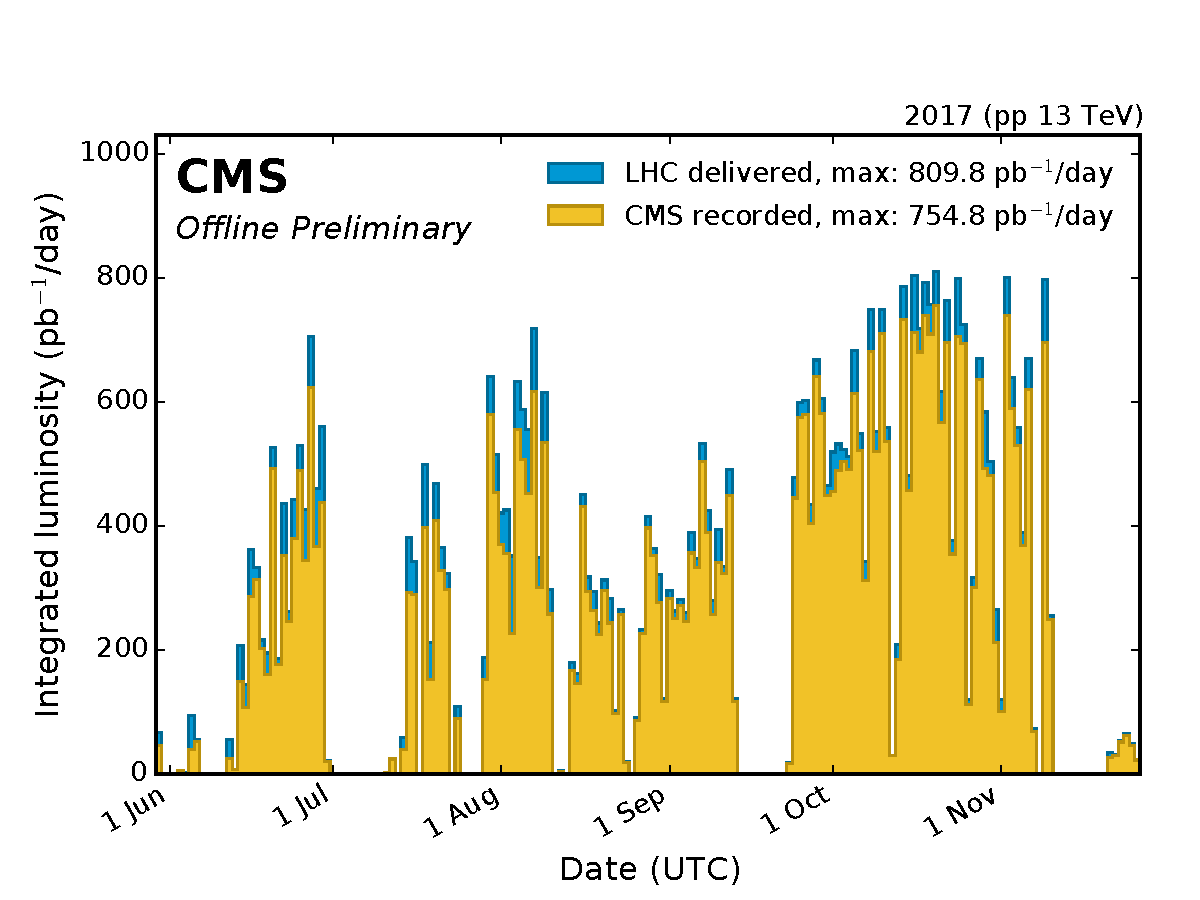
\includegraphics[width=.45\textwidth]{Chapter3/Luminosity/int_lumi_per_day_pp_2017_Normtag.pdf}
    \caption[Cumulative day-by-day integrated luminosity in 2017]{(Left) Cumulative daily integrated luminosity. (Right) Daily integrated luminosity, 2017.}
    \label{Lumi_2017}
\end{figure}

\begin{figure}[h!]
    \centering
    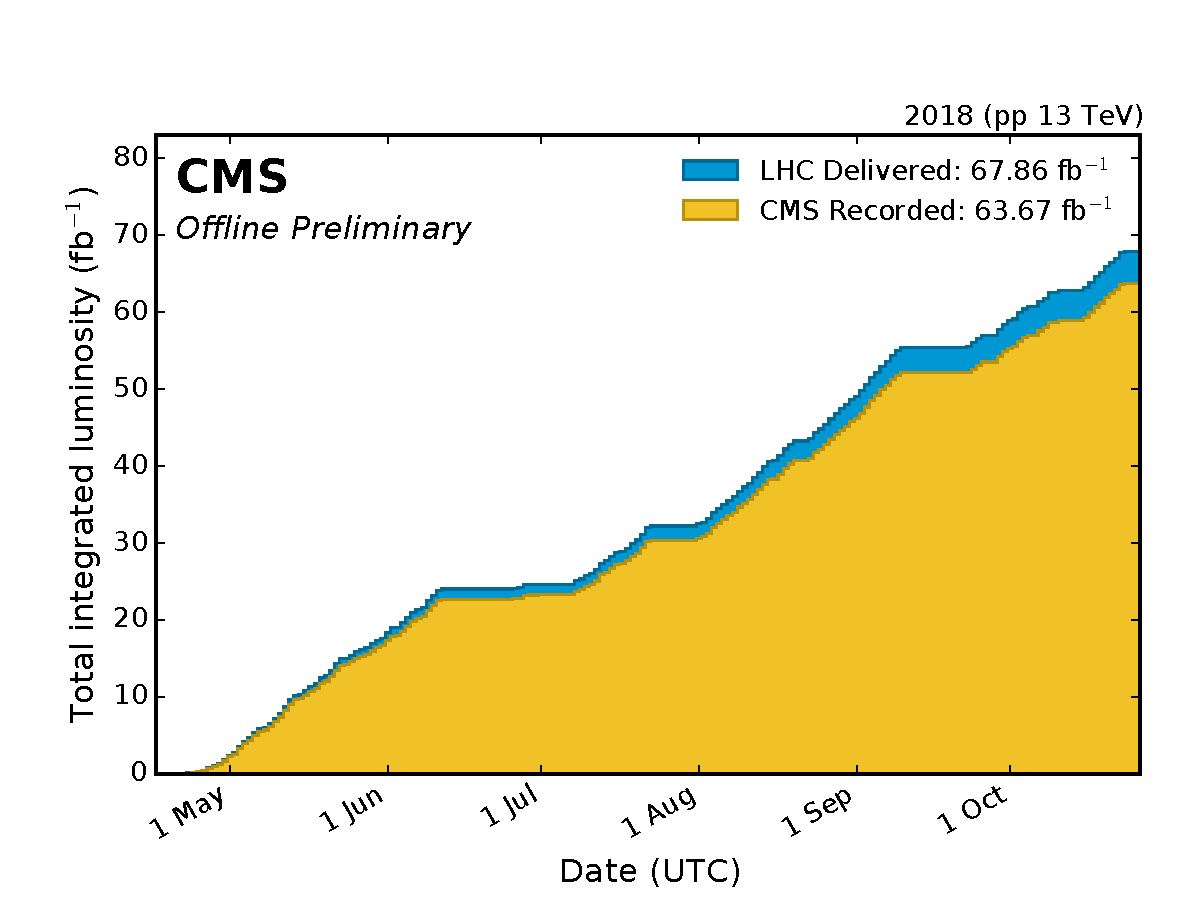
\includegraphics[width=.45\textwidth]{Chapter3/Luminosity/int_lumi_per_day_cumulative_pp_2018_Normtag.pdf}
    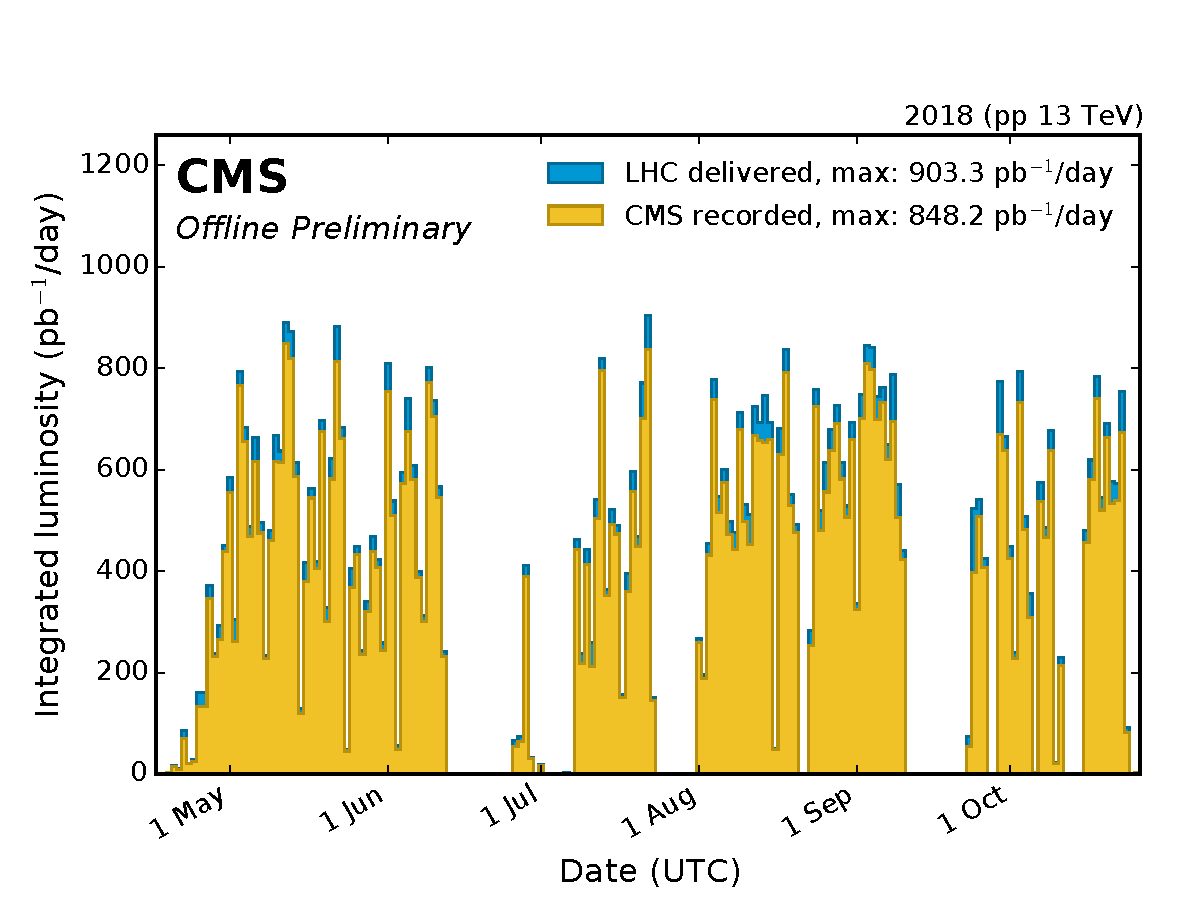
\includegraphics[width=.45\textwidth]{Chapter3/Luminosity/int_lumi_per_day_pp_2018_Normtag.pdf}
    \caption[Cumulative day-by-day integrated luminosity in 2018]{(Left) Cumulative daily integrated luminosity. (Right) Daily integrated luminosity, 2018.}
    \label{Lumi_2018}
\end{figure}

The Large Hadron Collider (LHC) operates in cycles known as fills, during which protons are injected, accelerated, and stabilized before collisions begin. Luminosity rises sharply after beam stabilization, reaching a peak before gradually decreasing due to proton depletion. The stable beams phase is when most data is collected. A fill ends when proton levels drop too low or technical issues arise, leading to a controlled beam dump and a sudden drop in luminosity.

Within each fill, data is recorded in runs, which represent continuous periods of data acquisition under stable detector and accelerator conditions. A single fill can contain one or more runs, depending on machine stability and configuration adjustments.

The Pixel Cluster Counting (PCC) physics data from each year is divided into datasets corresponding to specific time periods, defined by a range of runs. In 2017, five datasets were established: B, C, D, E, and F, with their respective run ranges listed in Table~\ref{tab:period_run_ranges_2017}. In 2018, the data was split into seven periods: A, B, C, D1, D2, D3, and D4, detailed in Table~\ref{tab:period_run_ranges_2018}.

\begin{comment}
\begin{table}[h!]
  \centering
  \caption[Run ranges for 2017 periods]{2017 luminosity data periods with run ranges.}
  \begin{tabular}{cc}
    \textbf{Period} & \textbf{Run range} \\ \hline
    2017B & 297046-299329 \\
    2017C & 299368-302029 \\
    2017D & 302031-302663 \\
    2017E & 303824-304797 \\
    2017F & 305040-306462 \\
  \end{tabular}
  \label{tab:period_run_ranges_2017}
\end{table}

\begin{table}[h!]
  \centering
  \caption[Run ranges for 2018 periods]{2018 luminosity data periods with run ranges.}
  \begin{tabular}{cc}
    \textbf{Period} & \textbf{Run range} \\ \hline
    2018A & 315252-316995 \\
    2018B & 317080-319311 \\
    2018C & 319337-320065 \\
    2018D1 & 320500-321665 \\
    2018D2 & 321710-322964 \\
    2018D3 & 323363-324420 \\
    2018D4 & 324564-325175 \\
  \end{tabular}
  \label{tab:period_run_ranges_2018}
\end{table}
\end{comment}

\begin{table}[h!]
  \centering
  \begin{minipage}[t]{0.45\linewidth}
    \centering
    \caption[Run ranges for 2017 periods]{2017 luminosity data periods with run ranges.}
    \begin{tabular}{cc}
      \textbf{Period} & \textbf{Run range} \\ \hline
      2017B & 297046-299329 \\
      2017C & 299368-302029 \\
      2017D & 302031-302663 \\
      2017E & 303824-304797 \\
      2017F & 305040-306462 \\
    \end{tabular}
    \label{tab:period_run_ranges_2017}
  \end{minipage}%
  \hspace{0.05\linewidth} % Espacio entre tablas
  \begin{minipage}[t]{0.45\linewidth}
    \centering
    \caption[Run ranges for 2018 periods]{2018 luminosity data periods with run ranges.}
    \begin{tabular}{cc}
      \textbf{Period} & \textbf{Run range} \\ \hline
      2018A & 315252-316995 \\
      2018B & 317080-319311 \\
      2018C & 319337-320065 \\
      2018D1 & 320500-321665 \\
      2018D2 & 321710-322964 \\
      2018D3 & 323363-324420 \\
      2018D4 & 324564-325175 \\
    \end{tabular}
    \label{tab:period_run_ranges_2018}
  \end{minipage}
\end{table}


The datasets used in the analysis are derived from the Alignment and Calibration (AlCa) project within CMS and include two subsets: Random Trigger and Zero-Bias. The Random Trigger dataset contains events triggered in both colliding and non-colliding bunches, while the Zero-Bias dataset consists of unbiased events randomly selected among colliding bunches, identified using the Beam Pick-up Timing for eXperiments (BPTX) system.

The Random Trigger data is reprocessed with an updated module veto list (as described in the next section) to improve background subtraction, known as afterglow corrections, which are further detailed in the next chapter. Similarly, the Zero-Bias dataset undergoes reprocessing with refined afterglow corrections to obtain the total yearly luminosity for PCC and to study stability and linearity in comparison with other luminometers.

In 2017, vdM program was conducted during period C (fill 6016), while in 2018, it took place during period B (fill 6868).


\section{Module selection}


The pixel detector experiences time-dependent variations in performance due to factors such as noise, aging, and radiation damage, which affect the number of well-performing modules. To maintain accurate luminosity measurements, a selection is applied to the 1856 pixel detector modules, retaining only those that remain stable and linear across different data-taking periods. Modules exhibiting instability, non-physical shifts in cluster counts, or significant effects from readout buffer limitations are excluded. This selection is based on each module’s relative contribution to the total statistics in standard physics runs, ensuring that only consistently performing modules are used in PCC rate measurements, thereby preserving measurement reliability.

To ensure accuracy, pixel module veto lists were generated for different time periods following the procedure described below for each year. These lists were processed using the data to improve both stability and linearity. Modules that were consistently identified as "bad" across multiple periods were excluded from the analysis. Finally PCC data with ZeroBias triggers was then reprocessed using this common veto list for final vdM analysis.

\subsection{2017 Pixel Detector module selection}
\label{sec:pcc_perf_moduleselection_2017}

%% Sam's presentation of the module veto: https://indico.cern.ch/event/704864/contributions/2891738/attachments/1599873/2536088/PCCUpdate20180213.pdf


The 2017 PCC data is divided into five periods (datasets) throughout the year: B, C, D, E, and F. The selection of stable ("good") detector modules is based on analyzing each module's cluster count relative to the total (module weight). The module weight is computed for each data period and compared across periods to assess stability.

During the final part of the 2017 run, power supply failures led to a significant number of non-operational modules, which were excluded from the final measurement. In particular, the Pixel detector experienced issues with DC-DC power converters during period F, resulting in a large number of unstable modules. Therefore, the stability analysis begins by comparing module weights between periods D and F.

Variations in module weight across periods are used to identify unstable modules. The selection threshold applied to the distribution ranged from 3\% to 5\%, depending on each pair of analysis periods. Table~\ref{tab:pcc_2017_module_selections} shows the number of modules that meet these criteria for every analyzed period pair.

\begin{table}[h]
    \caption{PCC 2017 detector module stability selections applied to the module weights}
    \label{tab:pcc_2017_module_selections}
  \begin{center}
    \begin{tabular}{cc}  
    \textbf{Periods}   & \textbf{\# Good modules} \\ \hline
     D + F      & 945           \\ 
     D + B      & 945           \\ 
     D + C      & 945           \\ 
     D + E      & 859           \\ 
     B + F      & 819          \\ 
     B + C      & 807          \\ 
     B + E      & 810          \\ 
     E + C      & 901          \\ 
     E + F      & 756          \\ 
     C + F      & 907          \\ \hline
     \textbf{Combined}   & \textbf{633}  \\ \hline
      \end{tabular}
  \end{center}
\end{table}


%The final list of good modules ("Combined") is obtained by requiring that modules be selected in all comparisons (i.e. the intersection of all sets).  Figure~\ref{fig:pcc2017modulevetofinal} shows the distribution of module weight ratios between periods B and D with the initial and final module selections, a large improvement is observed in the standard deviation of the distribution. 

\begin{comment}
\begin{figure}[h]
    \centering
    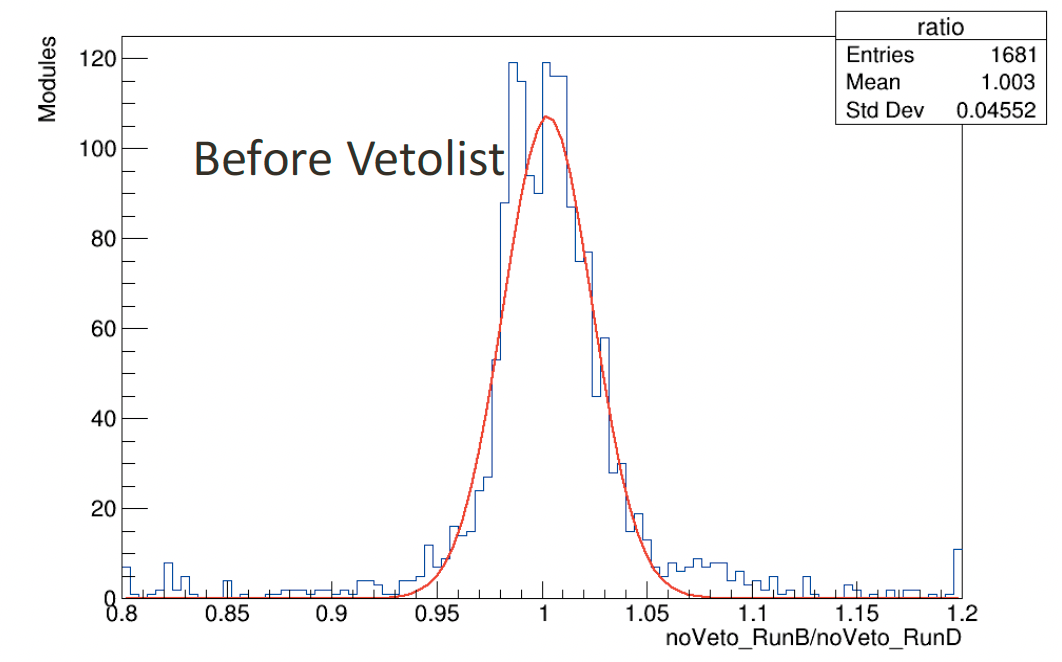
\includegraphics[width=0.48\textwidth]{figures/performance_PCC/PCC_2017_moduleveto_DB_initialveto.png}
    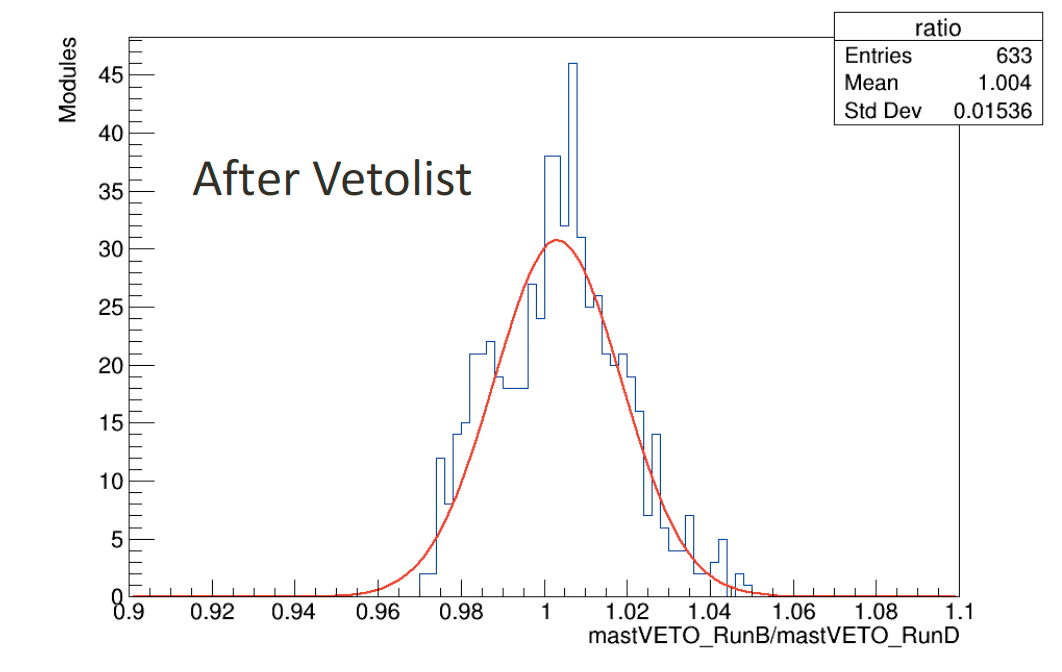
\includegraphics[width=0.48\textwidth]{figures/performance_PCC/PCC_2017_moduleveto_DB_finalveto.png}
    \caption{Distribution of module weight ratios for the 2017 periods B and D with the initial (left) and final (right) module selections.}
    \label{fig:pcc2017modulevetofinal}
\end{figure}
\end{comment}

The number of selected modules for the final analysis was \textbf{633 (34.1\%) for 2017}.


\subsection{2018 Pixel Detector module selection}
\label{sec:pcc_perf_moduleselection}


%[25] CMS Collaboration, “Description and performance of track and primary-vertex reconstruction with the CMS tracker”, JINST 9 (2014) P10009, doi:10.1088/1748-0221/9/10/P10009, arXiv:1405.6569

For the year 2018, the selection of good pixel modules is based on the analysis of ZeroBias data by evaluating the contribution of each module to the total cluster count (module weight). This method enables the identification and progressive removal of unstable modules through the analysis of fluctuations in their response. The data for this year is divided into seven periods: A, B, C, D1, D2, D3, and D4. The procedure applied to these periods is as follows.

First, the innermost pixel layer (Layer 0) is excluded from the analysis due to its known susceptibility to dynamic inefficiency at high instantaneous luminosity, where the readout chip becomes incapable of processing all incoming signals~\cite{pas_18}.

Then, a two-step selection is applied: initially, a 7\% cut is used to discard modules with large fluctuations. After recalculating the module weights using the updated sample, a refined 2\% cut is applied.

The vdM calibration data (Fill 6868), which belongs to period B, is treated first. Based on this dataset, an initial module veto list is constructed. The same procedure is then extended to the remaining periods—A, C, D1, D2, D3, and D4—using the results from period B as a reference. For each period, the two-step selection is repeated, and additional modules are excluded if their weight deviates by more than three standard deviations from the mean value observed in period B.

Figure~\ref{goodmodule} illustrates the Profile of good and bad modules and the stability profiles and RMS/mean distribution used for the selection.

\begin{center} \begin{figure}[h!] 
\centering 
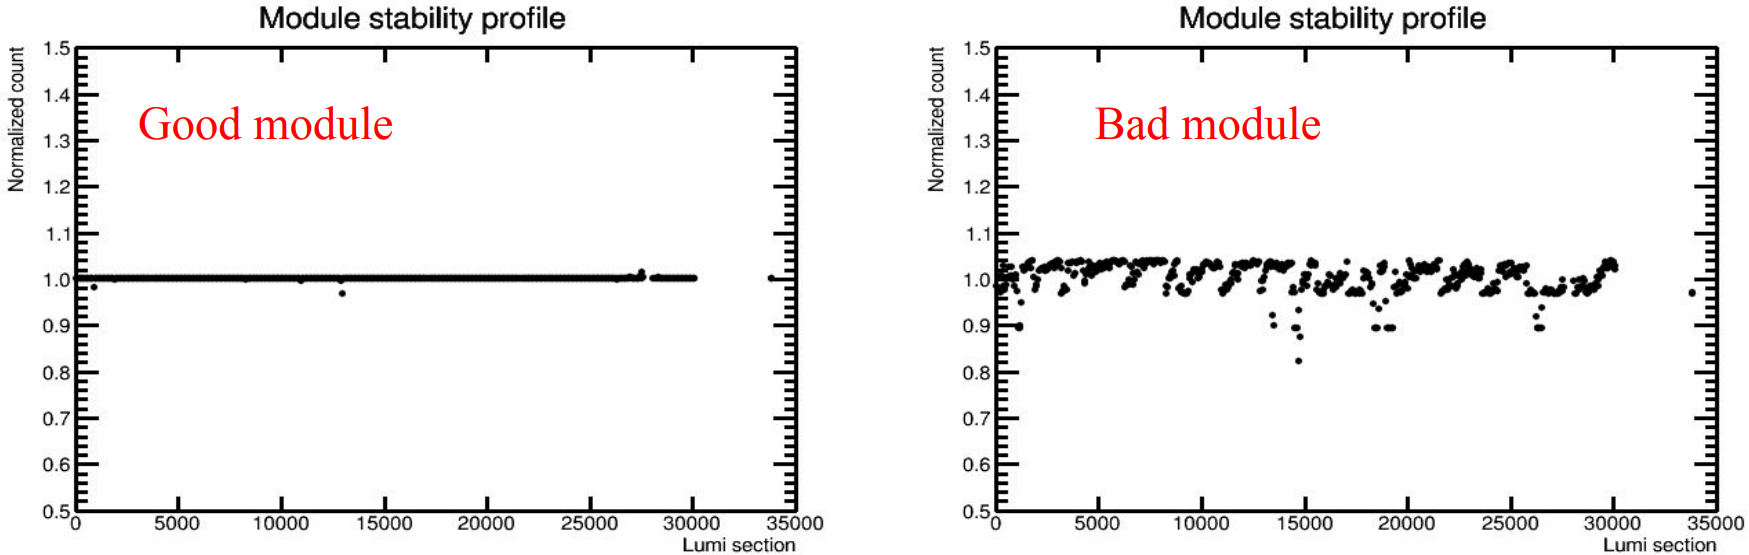
\includegraphics[scale=.17]{Chapter4/good_module.png}
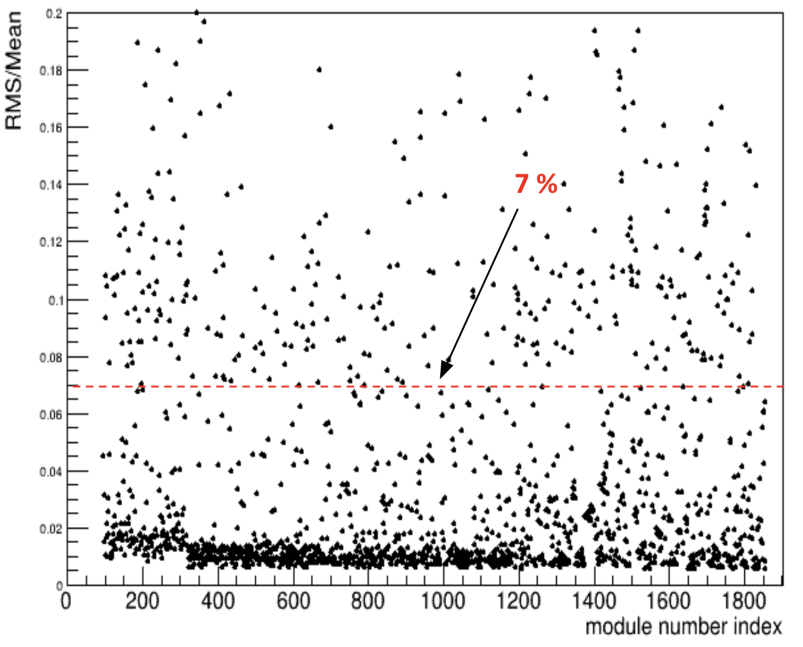
\includegraphics[scale=.15]{Chapter4/RMSmean.png} 
\caption[Profile of good and bad modules stability and module cut of 7\%]{Left: stability profiles of typical good and bad modules, showing the module weight as a function of lumi section. Right: RMS/mean values for all pixel modules, each represented by a module index. The 7\% cut is applied to this distribution in the first iteration.} \label{goodmodule} \end{figure} \end{center}


A common module list was created by combining all exclusive module lists from different period combinations. Table~\ref{tab:2commonveto} presents the number of good modules after sequentially combining each period.

\begin{comment}
\clearpage
\newpage
\begin{figure}[h]
    \centering
    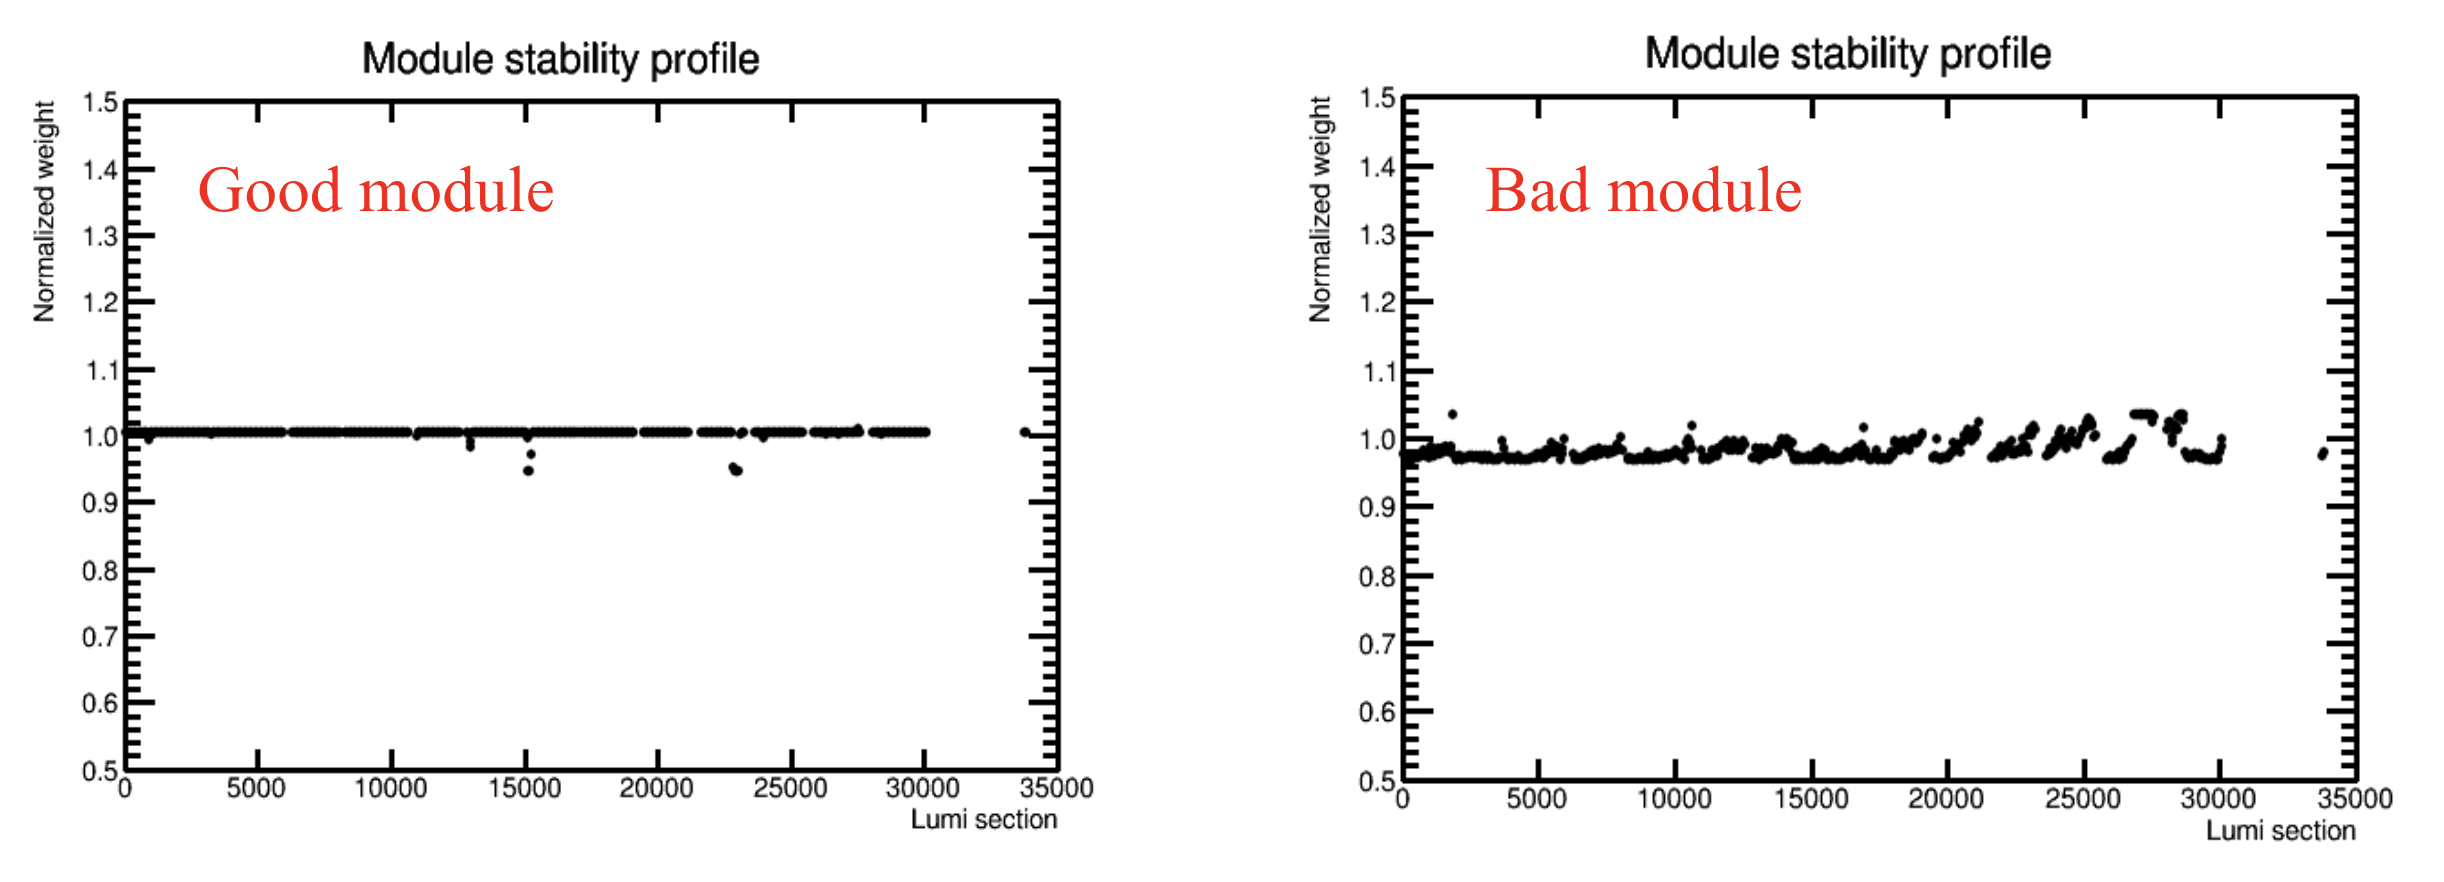
\includegraphics[width=1\textwidth]{figures/performance_PCC/good_bad_modules.png}
    \caption{Variation of normalized module weight with time. Modules showing significant change in module weight (shown in right figure) over time having large rms/mean values are used to make module vetolist.}
    \label{fig:goodbadmodules}
\end{figure}
\end{comment}

%\clearpage
%\newpage

\begin{table}[h]
\caption[Common Module Vetolist with Quality Selection]{Common module vetolist created by combining module vetolists for each period using a 2\% quality selection.}
    \label{tab:2commonveto}
  \begin{center}
    \begin{tabular}{ccccc}  
    \textbf{Period}   & \textbf{\# bad modules} & \textbf{\# good modules} \\  \hline
     B      &  802   &  1054    \\ 
     B + C      &  1076   &  780    \\ 
     A + B + C      &  1417   &  439    \\  
     A + B + C + D1      &   1534  &   322    \\ 
     A + B + C + D1 + D2      &   1629 &    227   \\ 
     A + B + C + D1 + D2 + D3     &   1668 &   188    \\ 
     A + B + C + D1 + D2 + D3 + D4     &  1701 &     155  \\ 
   \end{tabular}
  \end{center}
\end{table}


The number of selected modules for the final analysis was \textbf{155 (8.35\%) in 2018}. 

The relative contribution of each pixel detector layer and disk to the total PCC, after applying the final module selection, is shown in Fig.~\ref{fig:stabprof} as a function of time throughout the year.
%\includegraphics[scale=.17]
\begin{figure}[h]
    \centering
    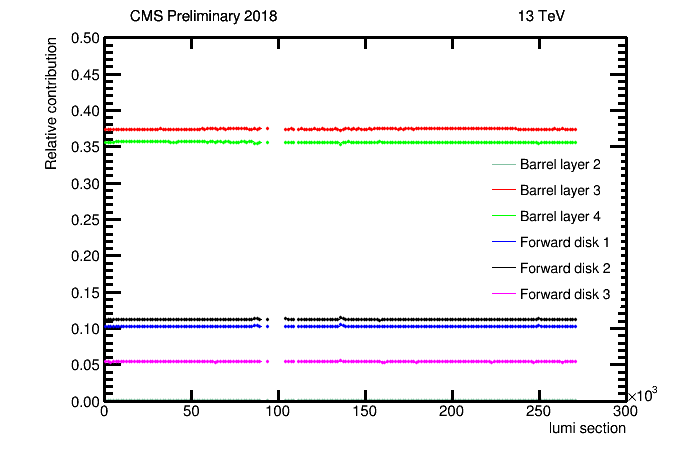
\includegraphics[width=0.7\textwidth, height=7cm]{Chapter4/module_selection/ProfileX_combined_testing_LUM_20-001.png}
    \caption[Stability Profiles of Pixel Layers and Disks After Final Module Selection]{Stability profiles of Pixel detector layers and disks with the final module selection.}
    \label{fig:stabprof}
\end{figure}

%Run range for each period is shown in Table \ref{tab:period run ranges}. 
 \begin{comment}
 Bad modules found after applying this 2\% selection in the final iterative step are used to constitute a 2 $\%$ rms module veto list for each period as shown in Table \ref{tab:per period veto}. 
                                                                                                           
\begin{table}
  \begin{center}
    \begin{tabular}{ccccc}  
    \textbf{Period}   & \textbf{\# bad modules} & \textbf{\# good modules} \\ \hline
     2018A      &   1276   &  580    \\  
     2018B      &    802  &     1054  \\ 
     2018C      &   1076  &    780   \\ 
     2018D1     &  1169  &     687  \\ 
     2018D2     &  1184  &    672   \\ 
     2018D3     &  1081  &    775   \\ 
     2018D4     &  1032  &     824  \\ 
      \end{tabular}
    \caption{2 \% rms module vetolist for each period showing number of good and bad modules.}
    \label{tab:per period veto}
  \end{center}
\end{table}
\end{comment}


\section{Afterglow Corrections}


The extended waveform of the signal recorded in silicon, along with the production of secondary particles from high-energy interactions with the detector material, defines the afterglow effects observed in PCC. The concept of afterglow is inherent to the detector and its recorded events, independent of the specific modules used for data collection. Consequently, a consistent afterglow correction is always necessary, regardless of module performance or operational state.

In precision PCC luminosity measurements, understanding and correcting afterglow effects is crucial. Afterglow corrections are estimated using a dedicated data stream recorded with a random trigger (raw PCC), as mentioned in the previous chapter. It is essential to use raw PCC data from both colliding and non-colliding bunches. Colliding bunches provide genuine signals from particle interactions, while non-colliding bunches capture background noise and any lingering afterglow from previous collisions. This data is collected at a total bandwidth of approximately 500 Hz, covering all bunch crossings in the LHC orbit. For analysis, the data is averaged over periods of approximately 50 lumisections (around 20 minutes). An example of raw data for Fill the 9036 is shown in Fig.~\ref{fig:af_fit40}.


\begin{figure}[H]
\centering
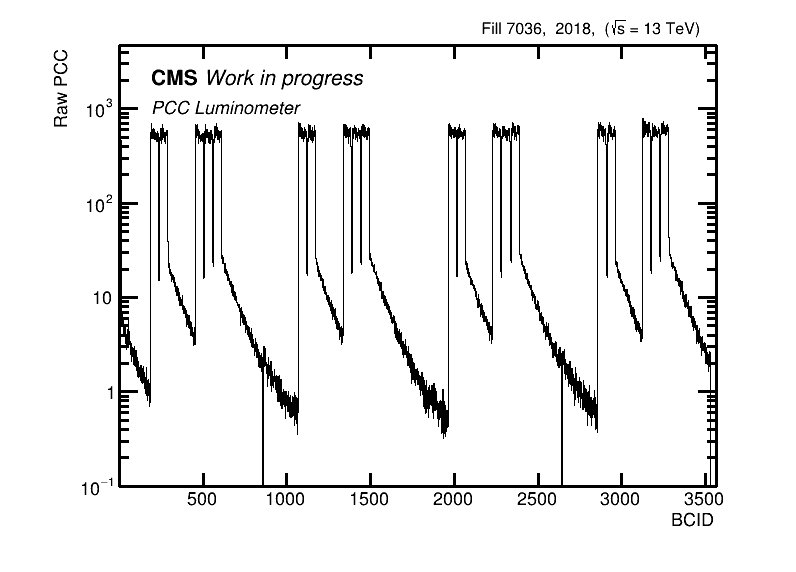
\includegraphics[width=0.8\textwidth]{figures/fill_7036_pattern_2.png}
\caption[7036 fill patern]{fill 7036,  and encompassing 900 colliding bunches, serves as the foundation for estimating the afterglow parameters.
}
\label{fig:af_fit40}
\end{figure}


Two main types of afterglow noise have been identified:

Type 1 Afterglow (Electronic Spillover): This noise originates from the prolonged signal waveform in silicon after a collision event.

Type 2 Afterglow (Activation-Induced Background): This exponentially decaying noise results from the activation of detector material by high-energy particles, leading to the production and decay of radioactive isotopes \cite{CMS-PAS-SMP-12-008}.

Both types can be observed in Fig.~\ref{fig:afterglow}.  

\begin{figure}[h]
    \centering
    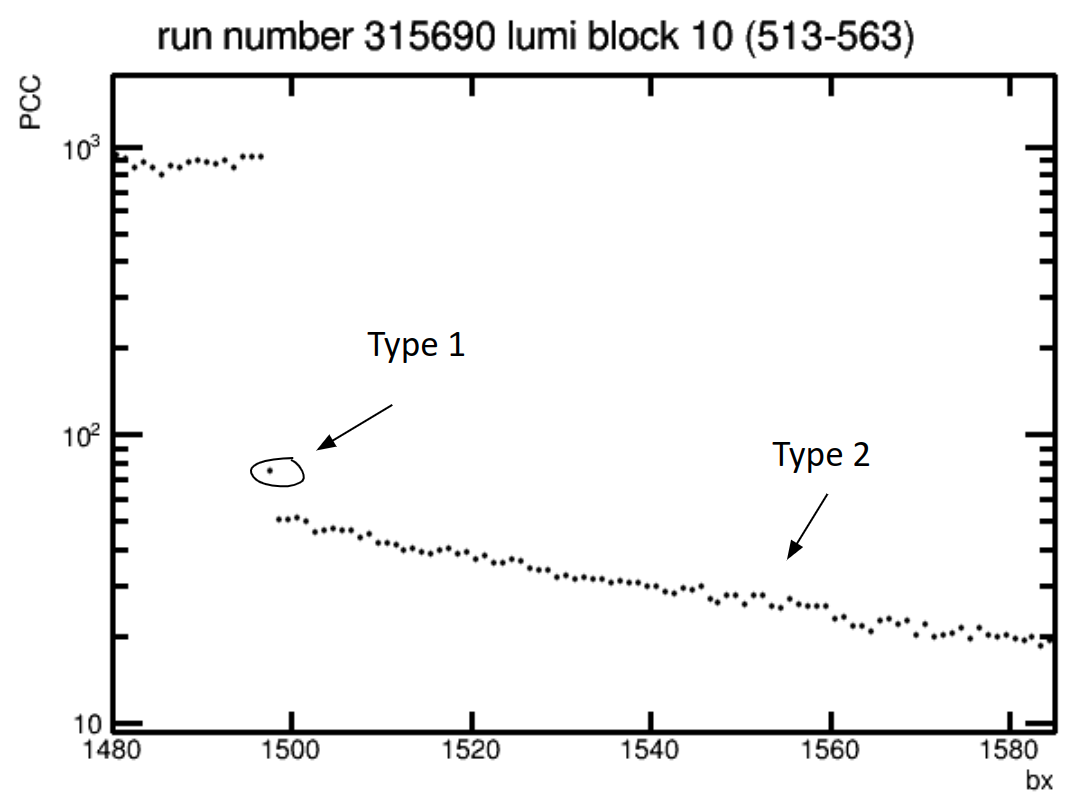
\includegraphics[width=0.6\textwidth]{figures/performance_PCC/afterglow.png}
    \caption[Type 1 and Type 2 Afterglow Responses in CMS Run 315690]{Train and afterglow tail showing type 1 and type 2 afterglow response in CMS Run 315690.}
    \label{fig:afterglow}
\end{figure}


In the afterglow correction process, the following steps are involved:

First, a mathematical fit function is used to model the afterglow tail from a single colliding bunch. This model incorporates parameters for Type 1 afterglow and an exponentially decaying function for Type 2, accounting for both amplitude and decay width. The function is summed over all bunch crossings and fine-tuned based on the luminosity associated with each bunch.tThe model expresses the amount of afterglow as follows:

\begin{equation}
F(x) = \sum_{k\in colliding } n_k \left[ \delta_{x,k} + A  \delta_{x,k+1} + B e^{-C(x - k - 1)}  \Theta(x-k-1) \right]
\end{equation}

Where $x$ is the BCID in the orbit, $k$ is an index over colliding bunches, $n_k$ is the cluster count for a colliding BCID excluding the afterglow and he first term $\delta_{x,k}$ corresponds to the colliding bunch. 
The term $A$ represents the Type 1 afterglow fraction (\( x = k+1 \)). For each 50 LS block, it is determined by iterating the model until a good fit to the data is achieved. This fraction, relative to the colliding bunch, is fitted in each block. 
and the last terms $B$ and $C$ corresponds to the Type 2 afterglow, which becomes relevant for $x\geq k+1$ and  are obtained from representative fills. This exponentially decaying component is characterized by two parameters: one for normalization relative to the colliding bunch rate and another for the decay constant. An example  for single train fit is shown in Fig. \ref{fig:af_fit99}. 

\begin{figure}
  \centering
    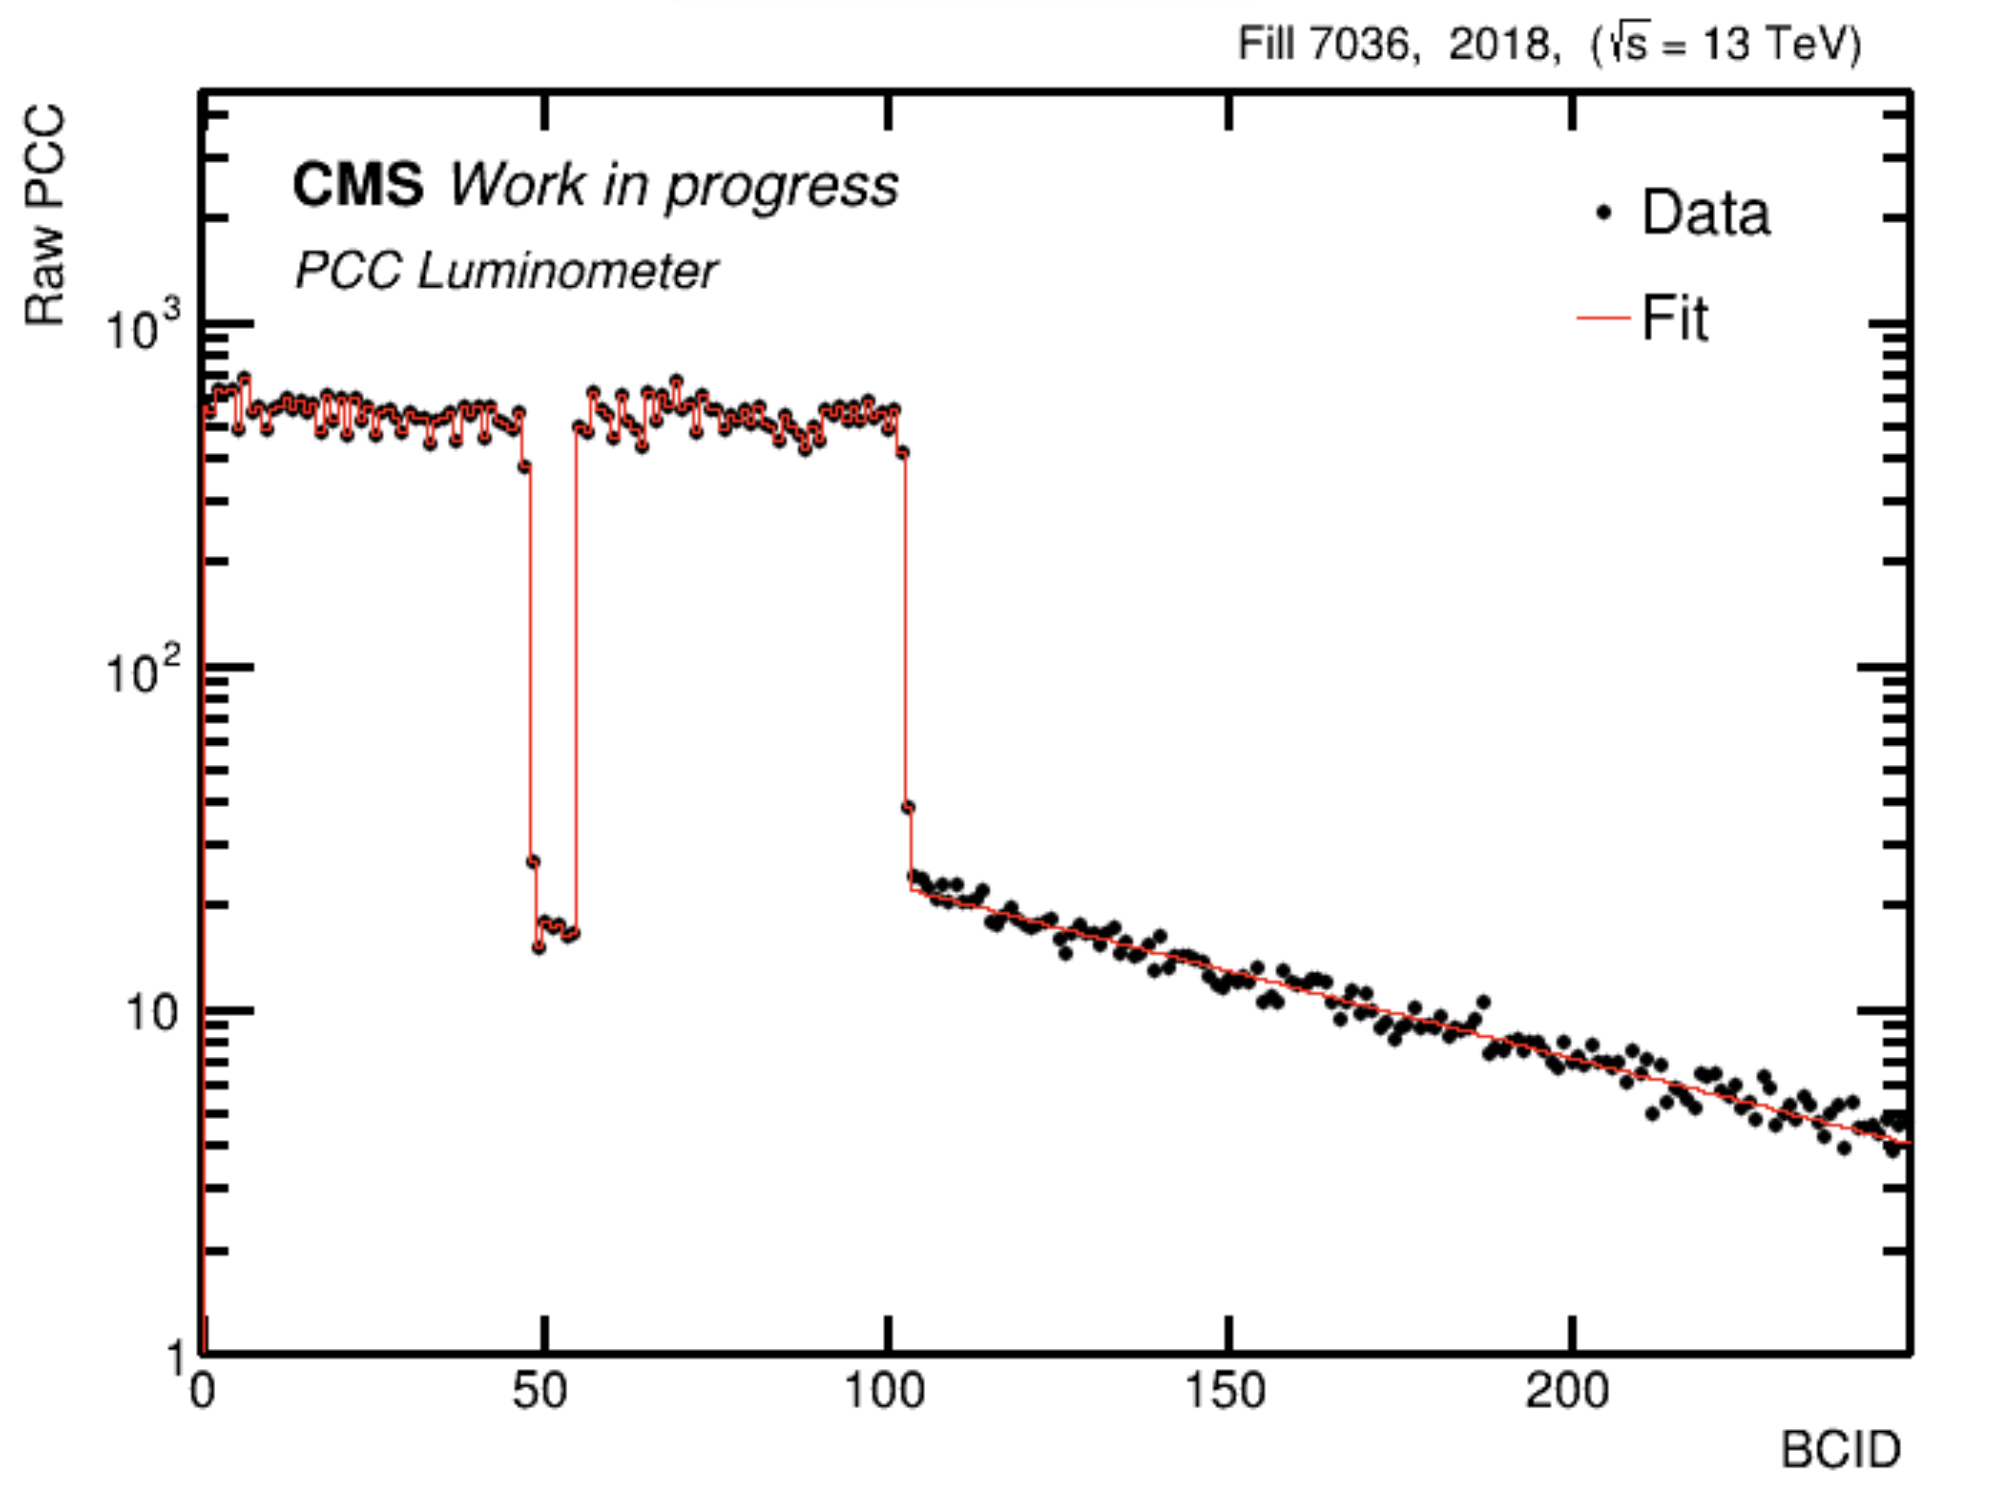
\includegraphics[width=0.75\textwidth]{figures/2018_af_fit_1.png} 
  \caption[Afterglow effect fit]{Fit to single train to estimate afterglow parameters.}
  \label{fig:af_fit99}
\end{figure}

\begin{comment}
Fig.~\ref{fig:pcc_type1f} shows the Type 1 parameter $A$ as a function of the PCC for both 2017 and 2018.

\begin{figure}[b]
    \centering
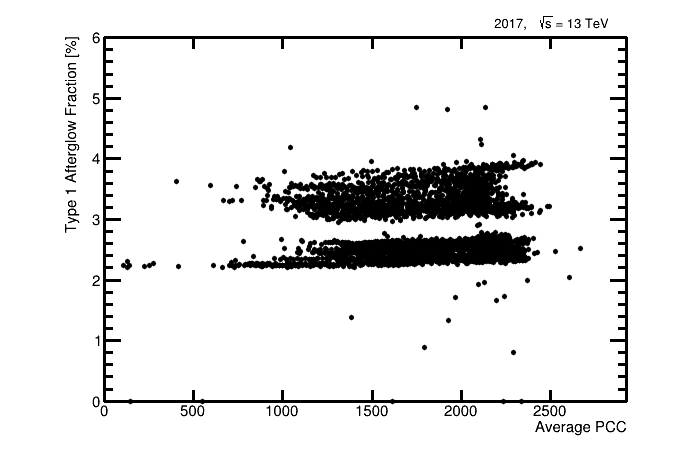
\includegraphics[width=0.48\textwidth]{figures/performance_PCC/afterglow_t1f_vsinstlumi_2017.png}
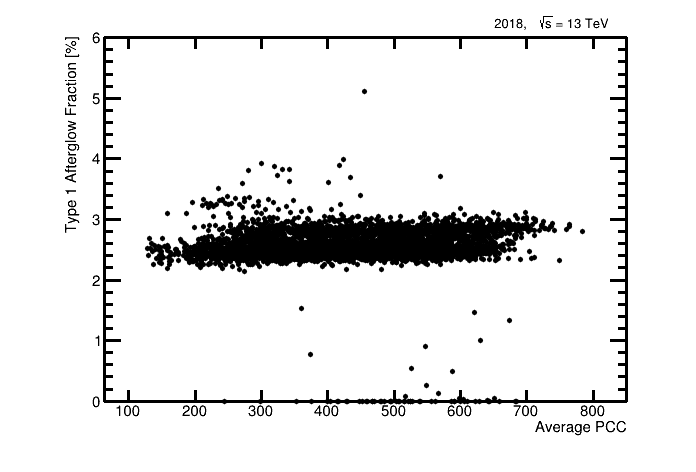
\includegraphics[width=0.48\textwidth]{figures/performance_PCC/afterglow_t1f_vsinstlumi_2018.png}
    \caption{PCC afterglow type 1 fraction as a function of PCC for the 2017 (left) and 2018 (right) datasets. Each point corresponds to one 50 LS block.}
    \label{fig:pcc_type1f}
\end{figure}


Fig. \ref{fig:pcc_residuals} shows the distribution residual counts in non-colliding BCID's relative to the average rate in colliding bunches. 

\begin{figure}
    \centering
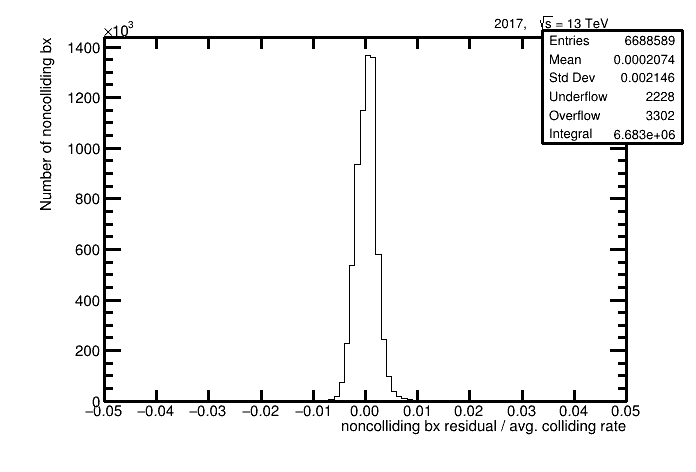
\includegraphics[width=0.48\textwidth]{figures/performance_PCC/afterglow_noncolliding_residual_2017.png}
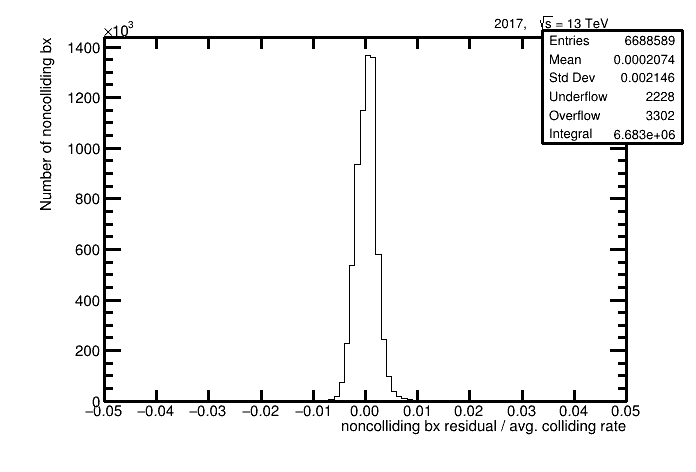
\includegraphics[width=0.48\textwidth]{figures/performance_PCC/afterglow_noncolliding_residual_2017.png}
    \caption{PCC afterglow residuals the 2017 (left) and 2018 (right) datasets. The distributions are filled with the residual cluster count in non-colliding bunches after subtracting the afterglow and dividing by the average cluster count in colliding bunches. The residuals are evaluated for blocks of 50 LS's.}
    \label{fig:pcc_residuals}
\end{figure}
\end{comment}


 The values of %of type 1 Fraction (A), 
 type 2 afterglow parameter amplitude (B) and decay width (C) for both years are shown in Table \ref{fig:af_fit4000}.

%\FloatBarrier
\begin{table}[H]
  \centering
  \caption[Type 2 afterglow parameters estimation]{Type 2 afterglow parameters obtained from fit to raw pcc data for both years}
  \begin{tabular}{ccc}
    \textbf{year} & \textbf{B} & \textbf{C} \\
     \hline
   %1-wagon train  & 0.001246  & 0.01261 \\
   2017  & 0.0008228 &  0.01316\\
   2018  & 0.0008265 &  0.01231\\
  \end{tabular}
  %\caption{Type 2 afterglow parameters obtained from fit to raw pcc data}
  \label{fig:af_fit4000}
\end{table}


The afterglow correction is determined by the ratio of corrected to uncorrected PCC, which serves as a scale factor applied to individual bunch-by-bunch histograms in the zero-bias data. Figure \ref{fig:afterglowcorrection} illustrates this scale factor for a 50-lumi-section block in run 315690. On the left, both the Random PCC data and corrected PCC values are shown for all bunch crossings, highlighting the differences between the initial data and the adjusted counts. On the right, the afterglow scale factor for a single 50-lumi-section block is displayed, representing the correction applied for the final module veto.


\begin{figure}[H]
    \centering
    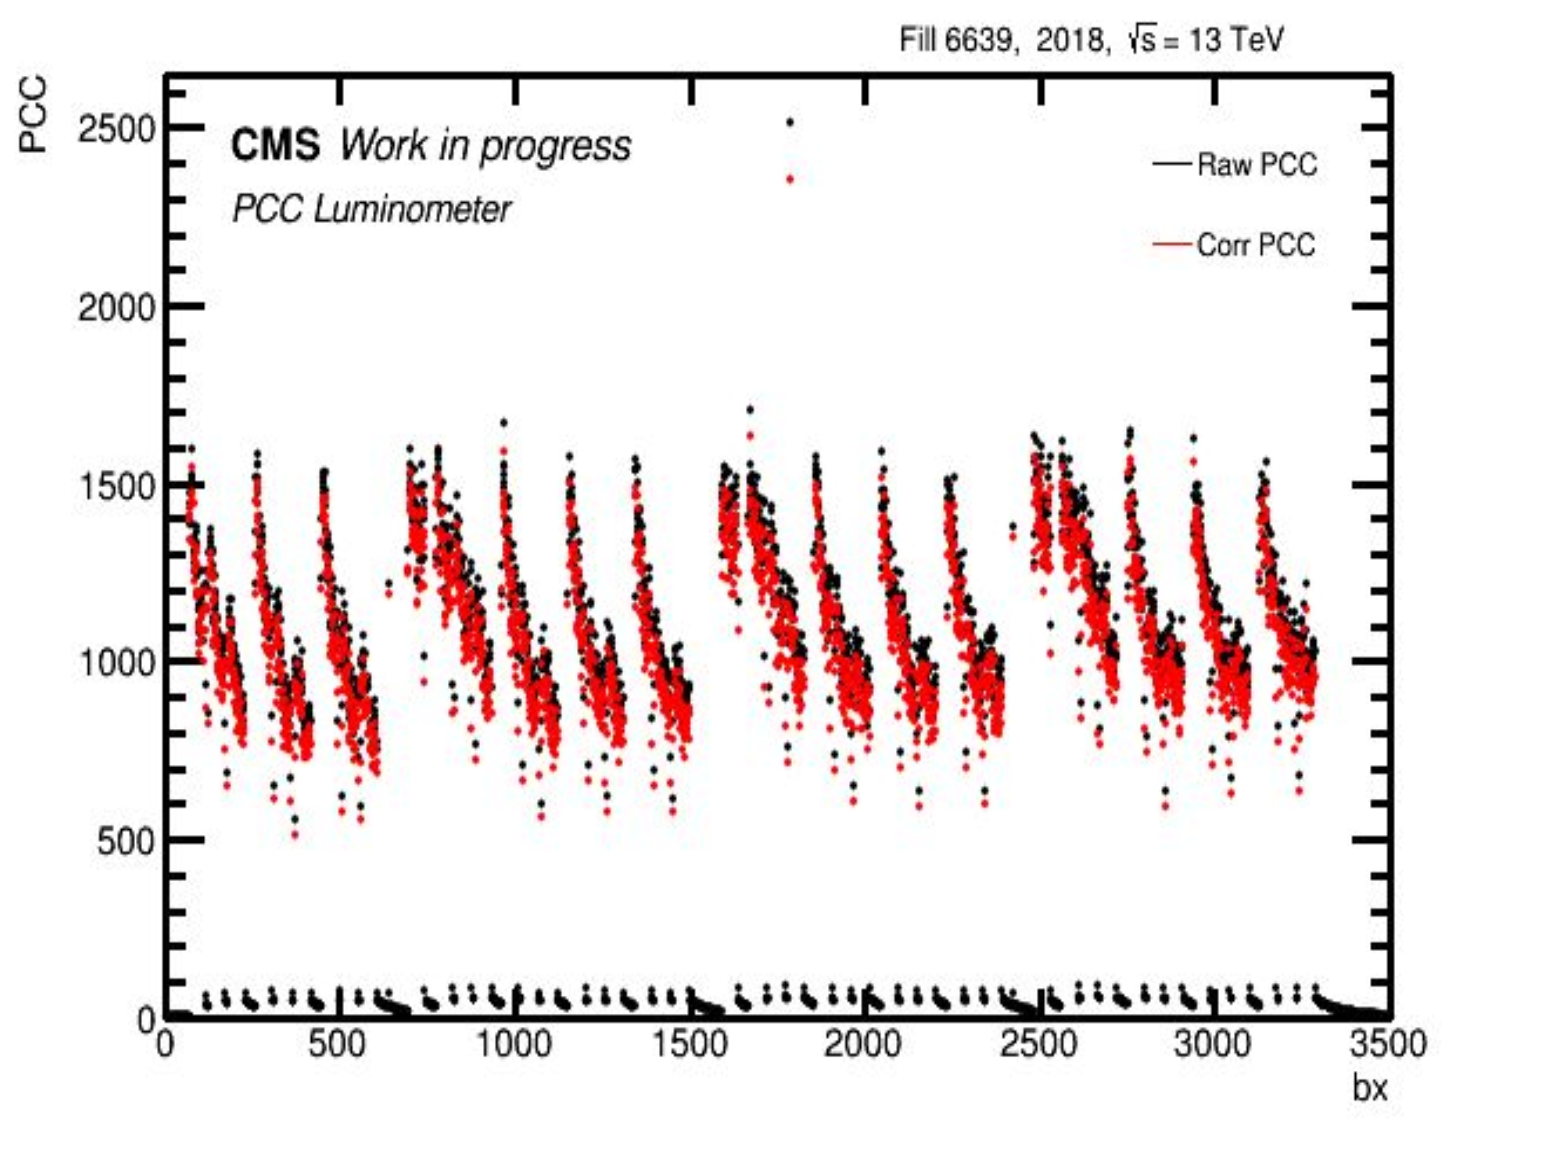
\includegraphics[width=0.48\textwidth]{figures/performance_PCC/afterglow_correction_factor_1lsblock_315690_2.png}
    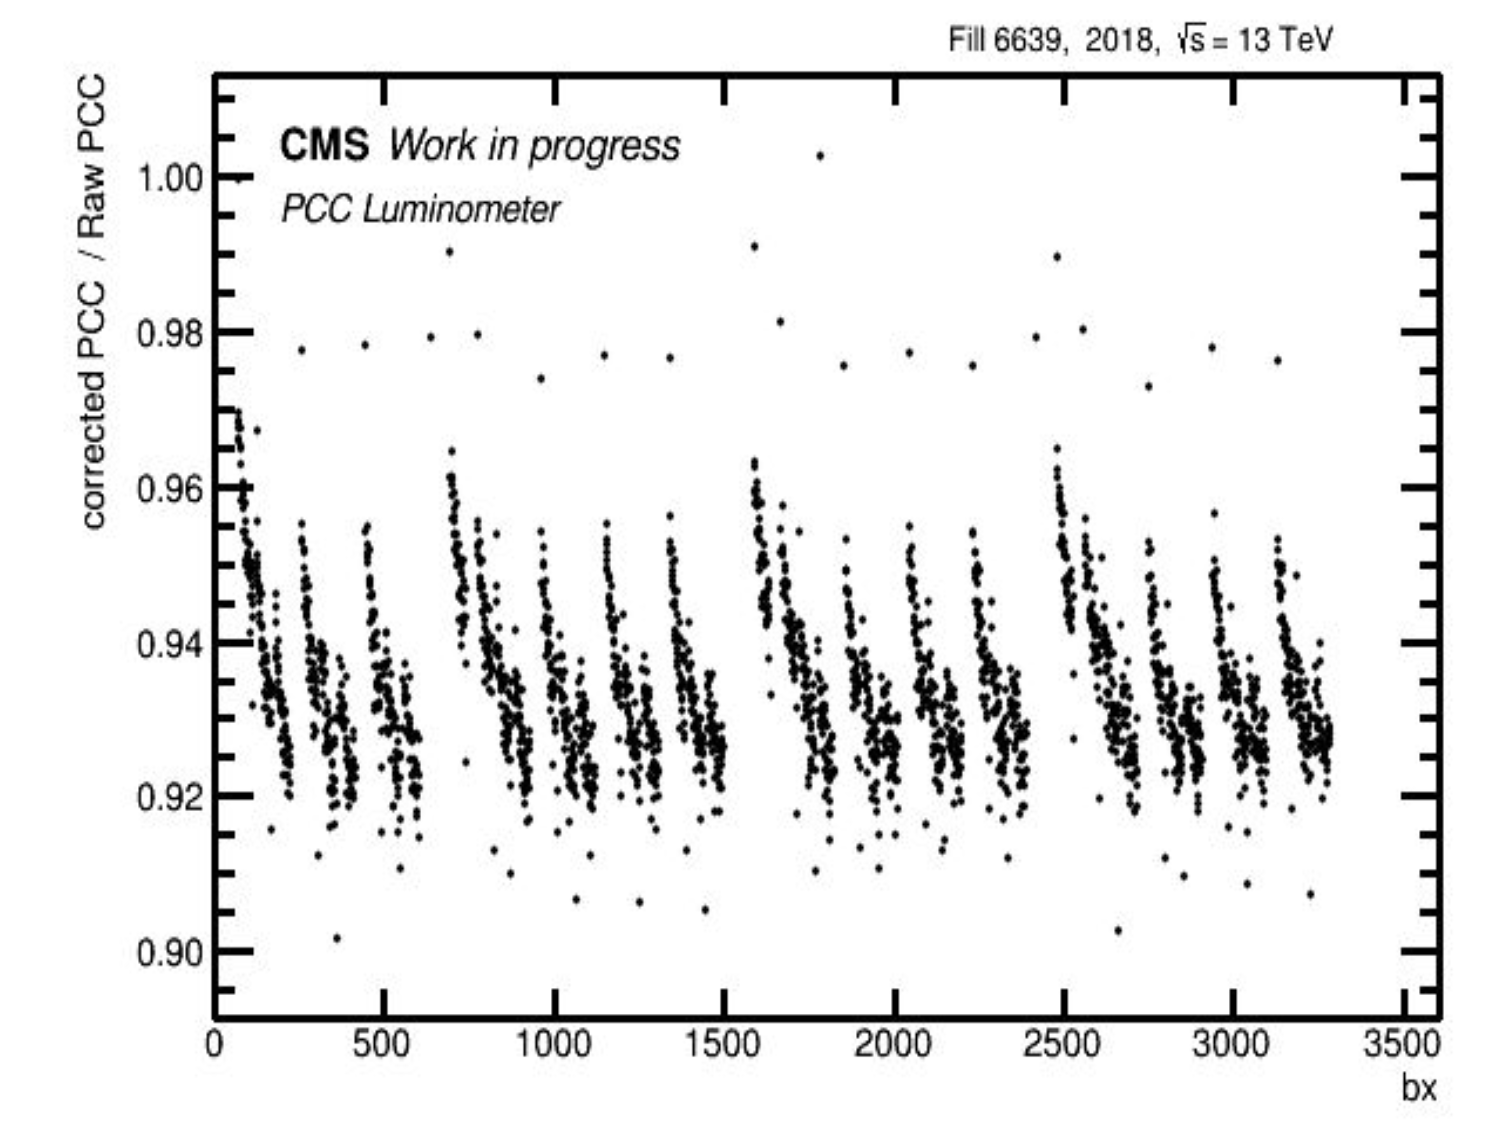
\includegraphics[width=0.48\textwidth]{figures/performance_PCC/afterglow_correction_factor_1lsblock_315690_3.png}
    \caption[PCC Random Rates vs BCID Before and After Afterglow Subtraction (Fill 6639)]{Left: PCC Random rates vs BCID for one 50 LS block in fill 6639 before and after the afterglow subtraction. Right: The ratio of raw and afterglow corrected rates, these ratios are applied to the ZeroBias data for the luminosity measurement.}
    \label{fig:afterglowcorrection}
\end{figure}


During the correction process, a histogram of collision events, including bunch trains, is adjusted by subtracting the afterglow model, scaled by the luminosity of each colliding pair, from all subsequent events. This ensures that each bunch is fully corrected. Finally, the correction scale factor is defined as the ratio of corrected to uncorrected PCC and is applied to the final PCC in the zero-bias (ZB) data.



\begin{comment}

Figure~\ref{fig:pcc_afterglow} shows per-bunch pixel cluster counts per event from a 2018 fill before and after the application of the OOT corrections in the vicinity of the last bunch train before the abort gap: the increased contribution from spillover is clearly visible for the first bunch after the train on top of the exponential activation tail.



\begin{figure*}[htbp]
    \centering
    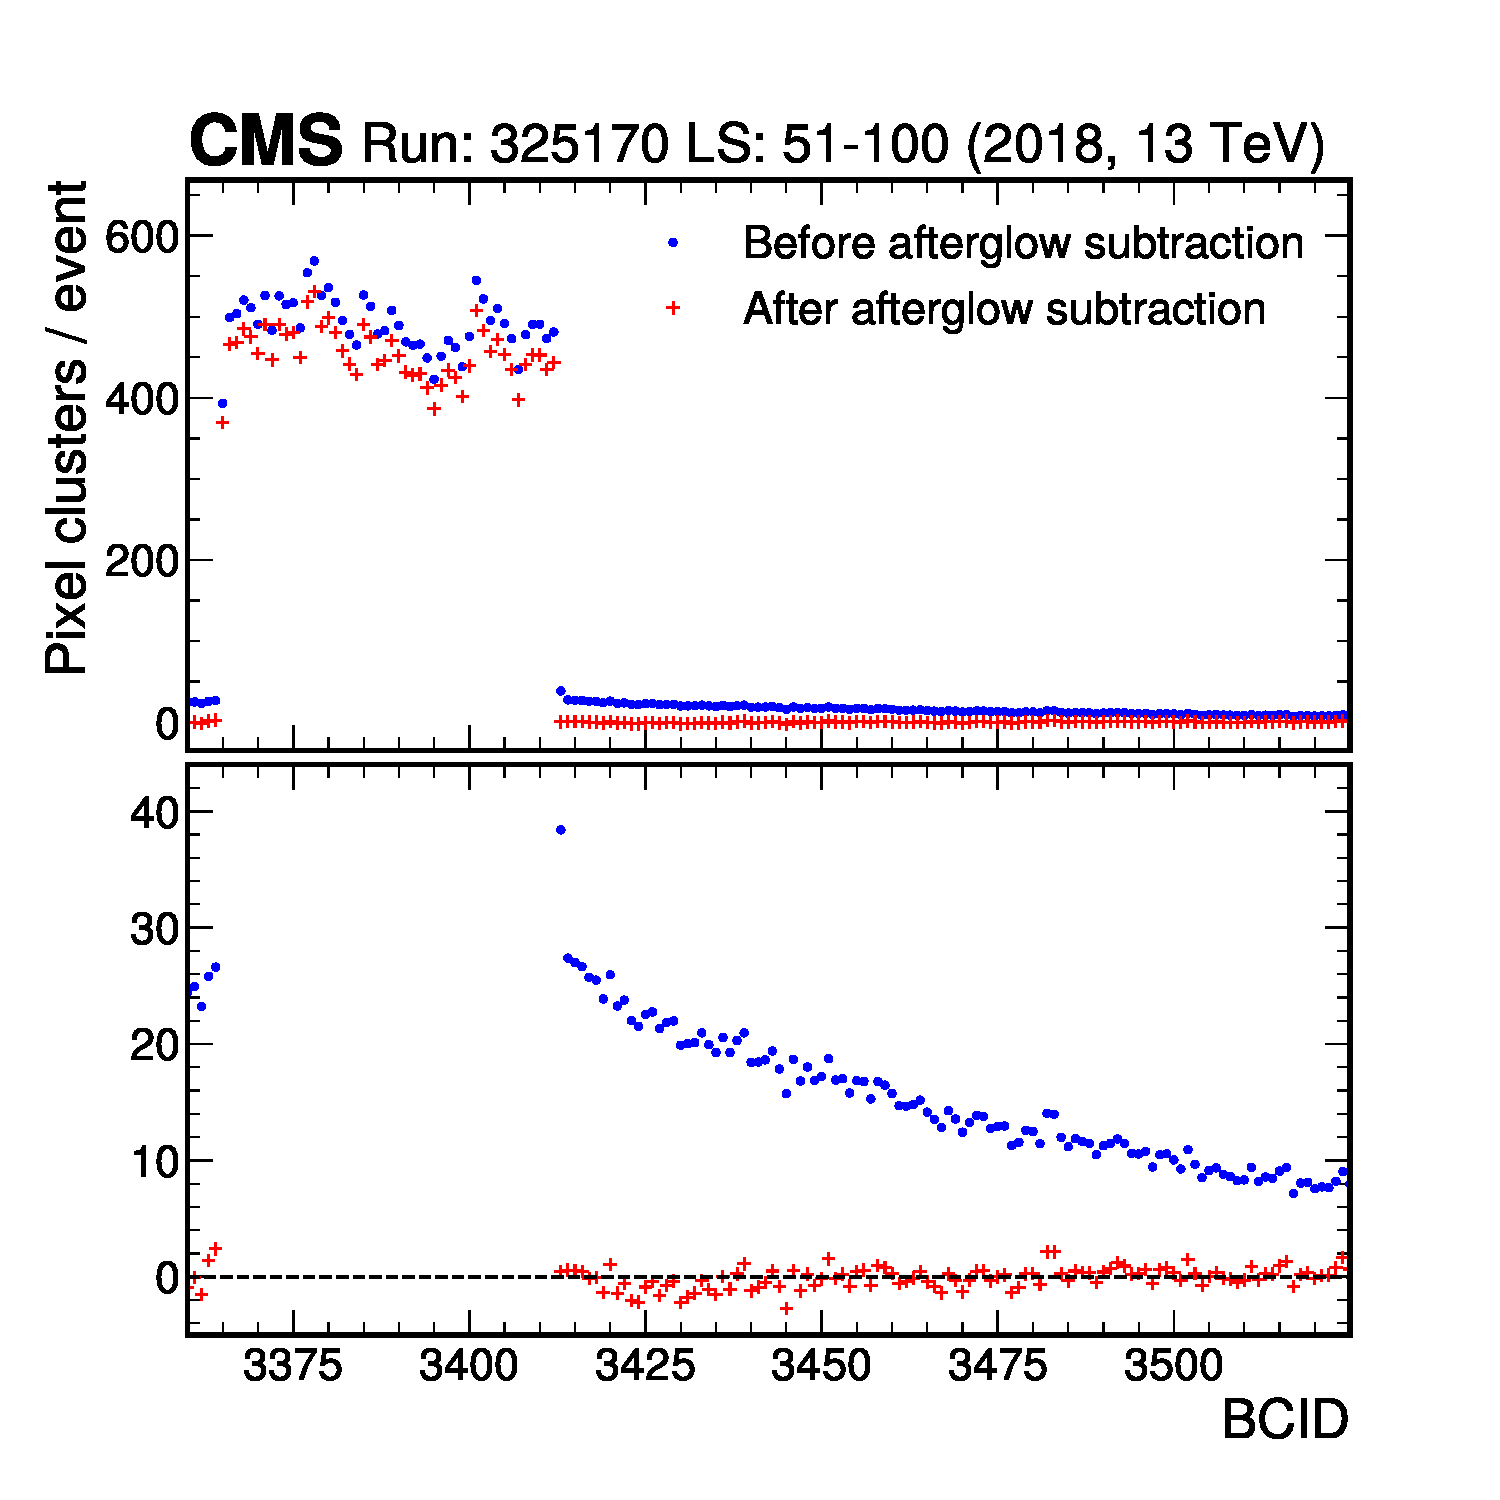
\includegraphics[width=0.66\textwidth]{figures/detector_corrections/PCCAfterglow_zoomed_range.pdf}

\caption{The number of clusters in the pixel tracker per event as a function of the BCIDs for the last bunch train of the orbit, with blue points representing the values before, and red crosses showing the results after the out-of-time corrections are applied. The upper panel focuses on the full count range for colliding and empty BCIDs, while the lower panel shows the empty bunch crossings with a different scale for better visibility. In the lower panel, the red crosses indicating the residual rate are near zero, illustrating the excellent performance of the correction.}
\label{fig:pcc_afterglow}
\end{figure*}


\begin{figure}
    \centering
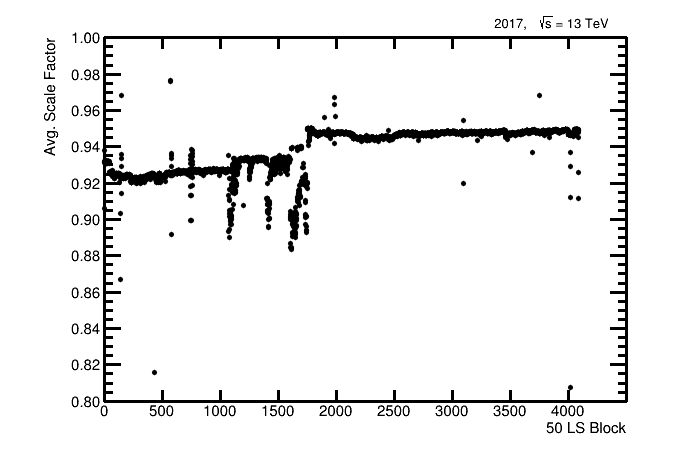
\includegraphics[width=0.48\textwidth]{figures/performance_PCC/afterglow_avgsf_vsLSBlock_2017.png}
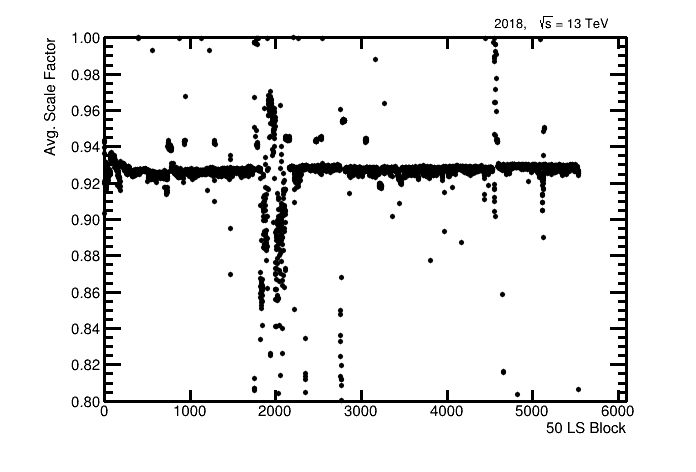
\includegraphics[width=0.48\textwidth]{figures/performance_PCC/afterglow_avgsf_vsLSBlock_2018.png}
    \caption{PCC average afterglow scale factors per orbit for the 2017 (left) and 2018 (right) datasets. Each point corresponds to one 50 LS block time ordered during the year.}
    \label{fig:pcc_afterglow_avgsf}
\end{figure}

\end{comment}



\section{Luminosity integration}
\label{sec:luminosity_integration_and_uncertainty}

The luminosity integration entails applying the afterglow correction and the absolute vdM calibration to the luminometer rates, with all corrections applied as described in Sec. \ref{bbcorrections} over a full year of physics data-taking. These yearly datasets, collected for each luminometer, are used to estimate systematic uncertainties related to cross-detector consistency (stability) and linearity.

An example of the calibrated instantaneous luminosity for PCC in 2017 is shown in Fig. \ref{Lumi_2017}. The plot on the left displays the calibrated Instantaneous luminosity throughout the entire year where data is presented as discrete measurements for each lumi section, reflecting the collision rate at that specific time. On the right, the luminosity evolution for a single fill (Fill 6120) is shown, where the gradual decrease in luminosity over time is clearly visible, this decline results from the loss of protons as collisions take place during the fill.


\begin{figure}[h!]
    \centering
    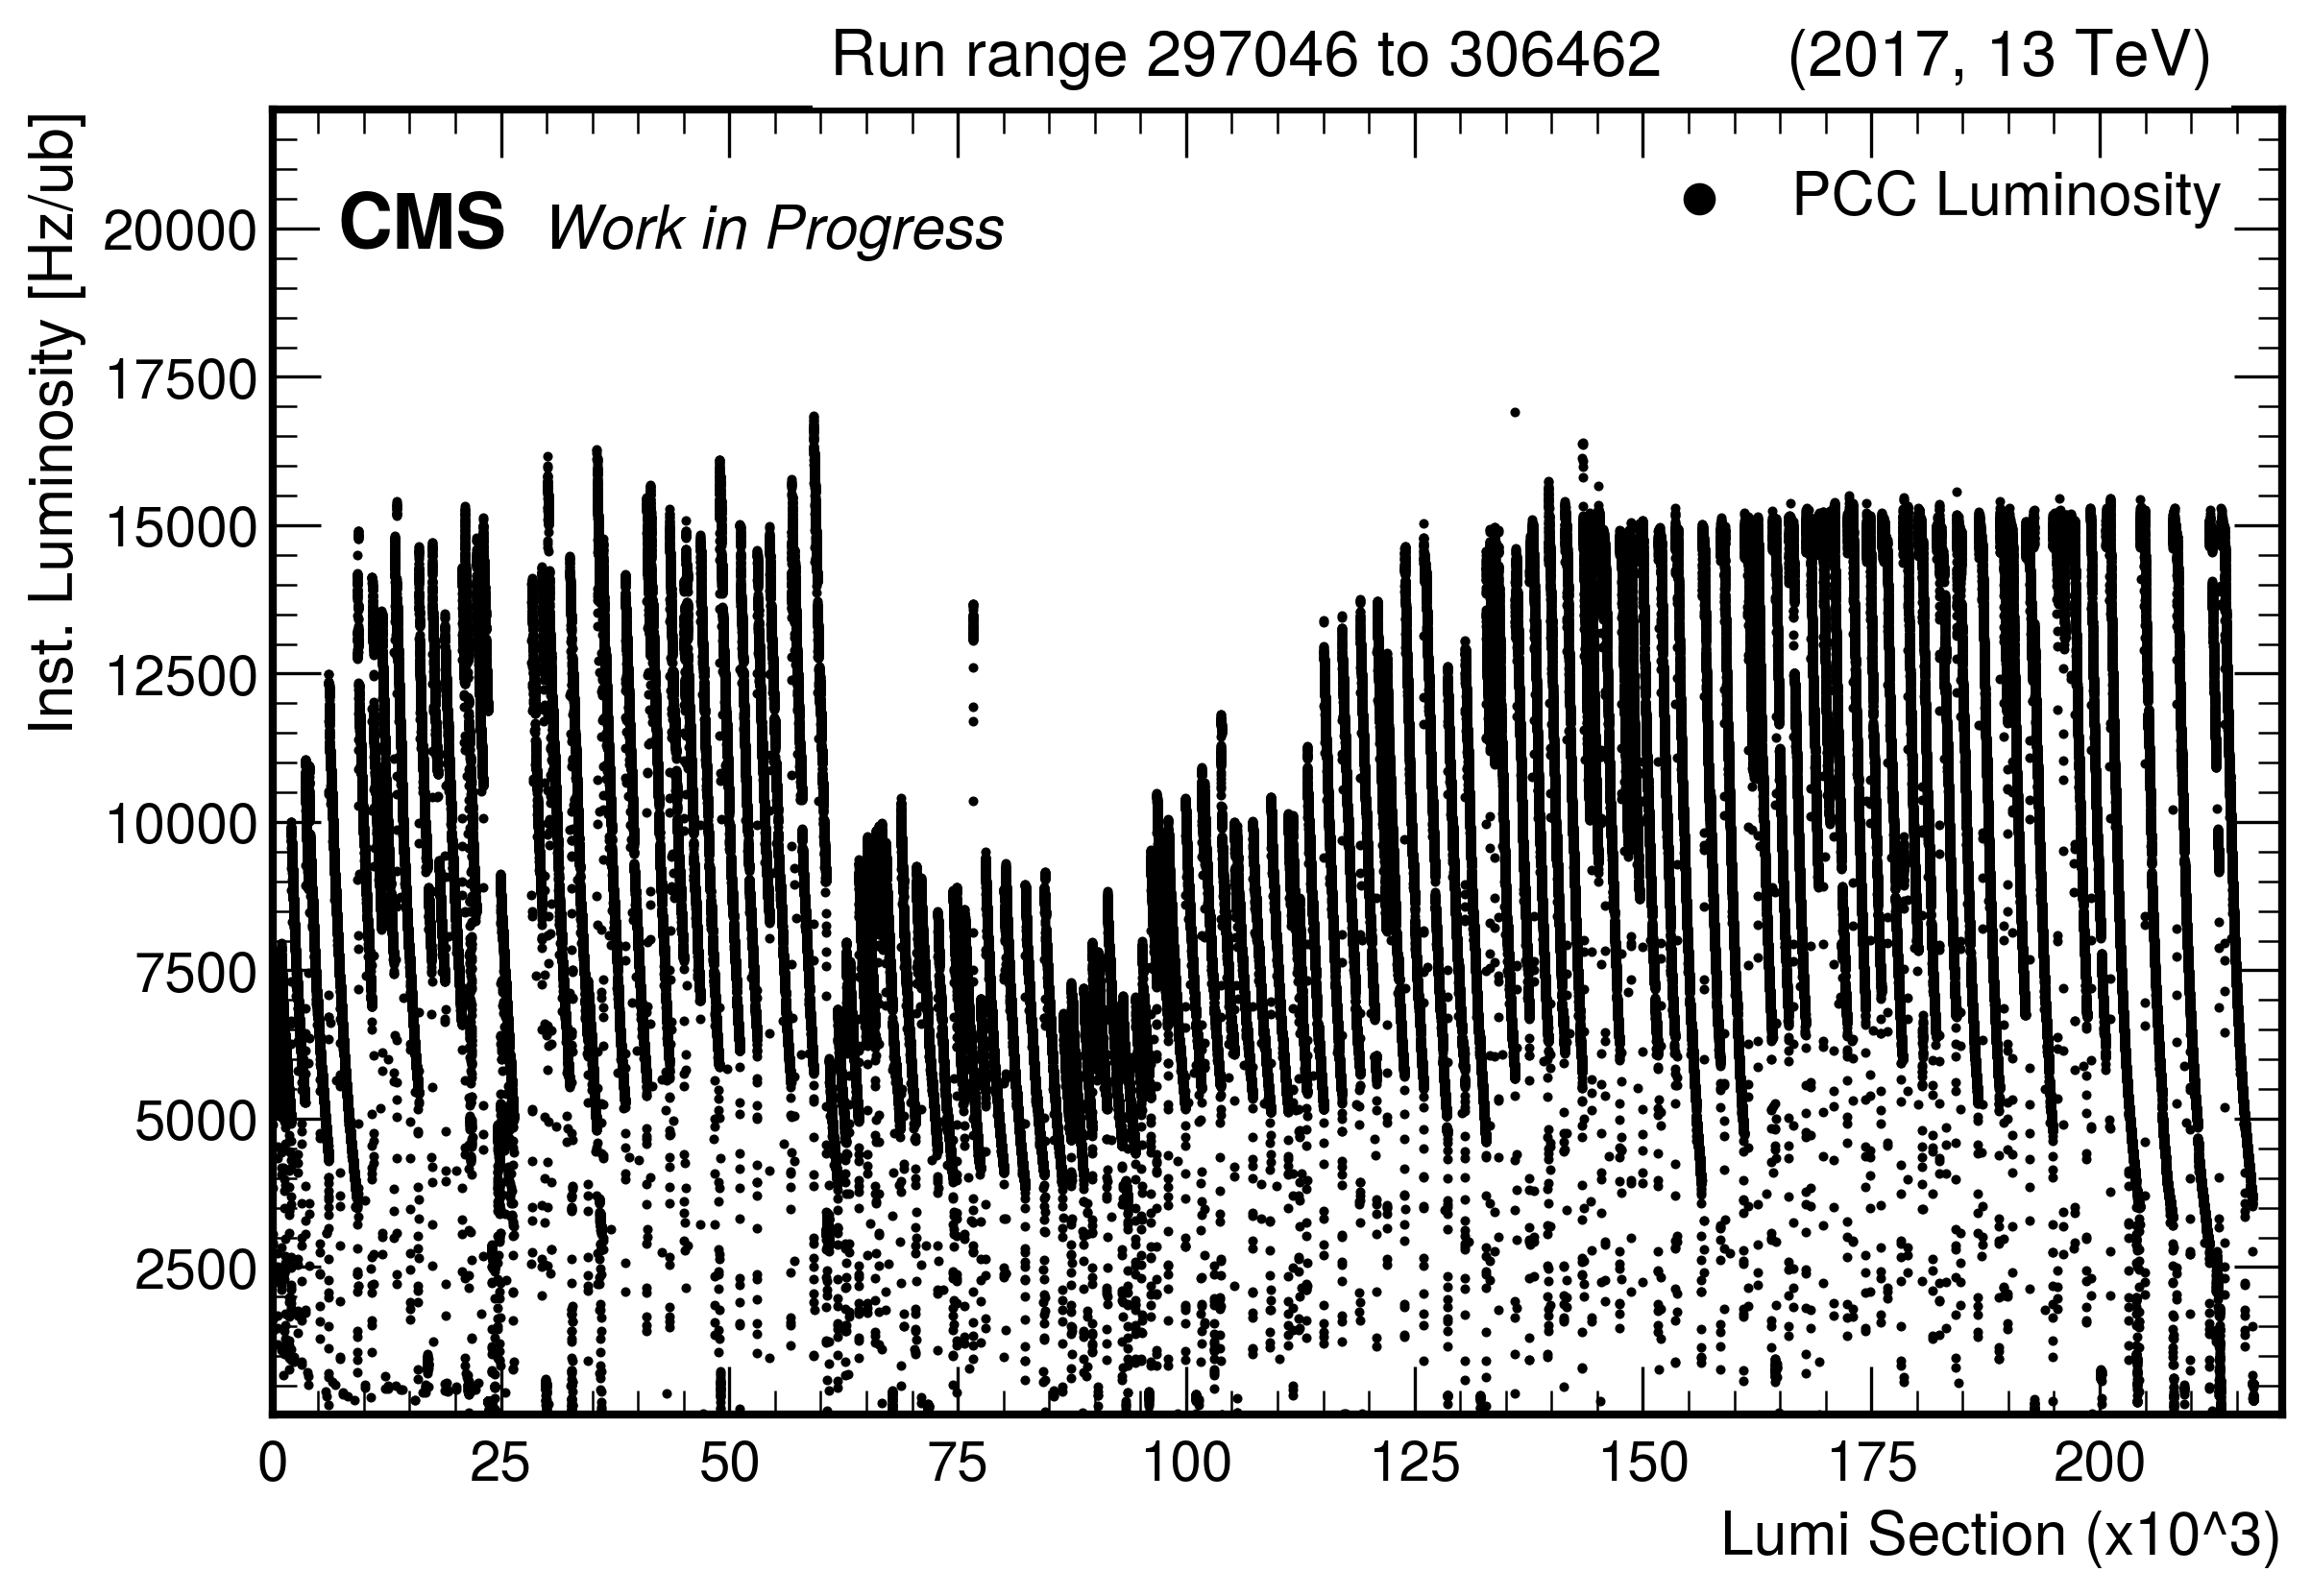
\includegraphics[width=.47\textwidth]{figures/performance_PCC/Lumi_2017.png}
    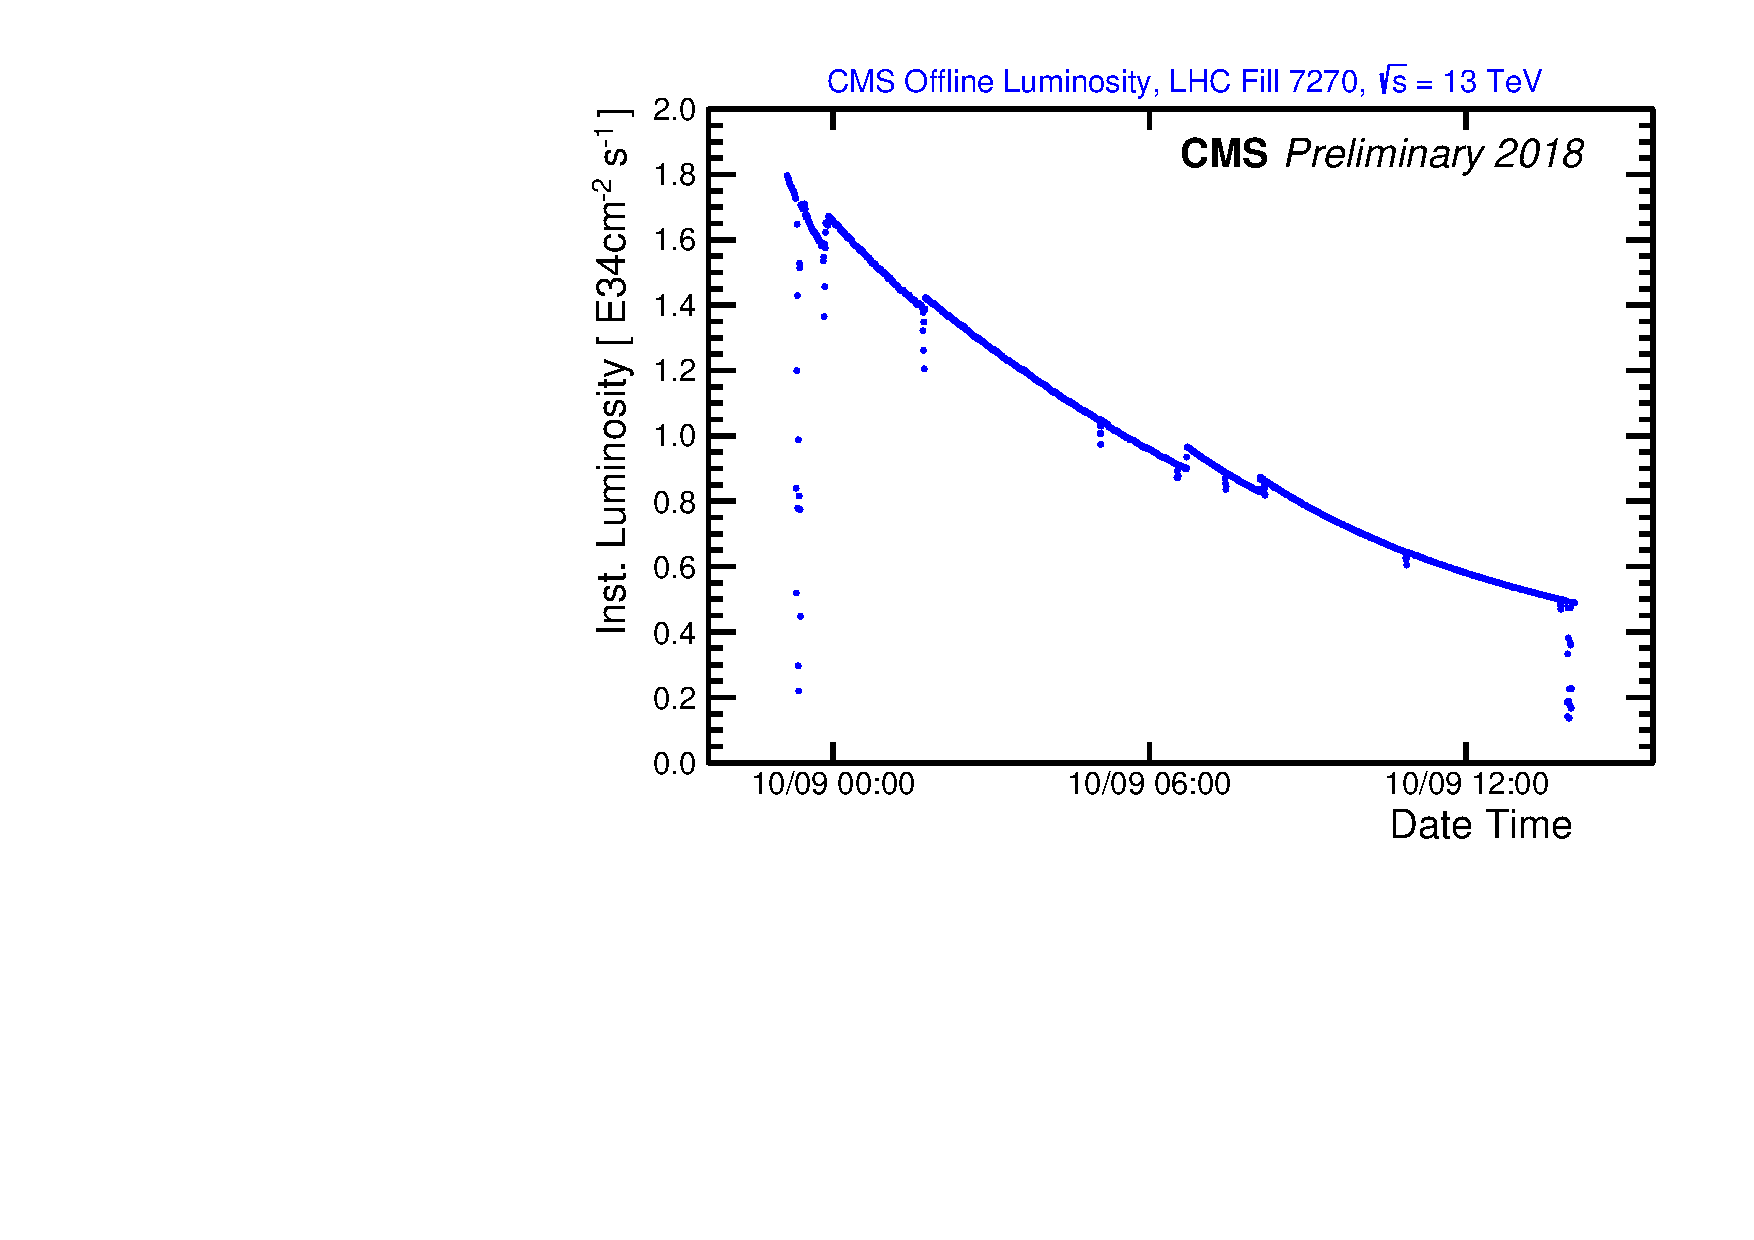
\includegraphics[width=.45\textwidth]{figures/LumiVsTime_fill7270.pdf}
    %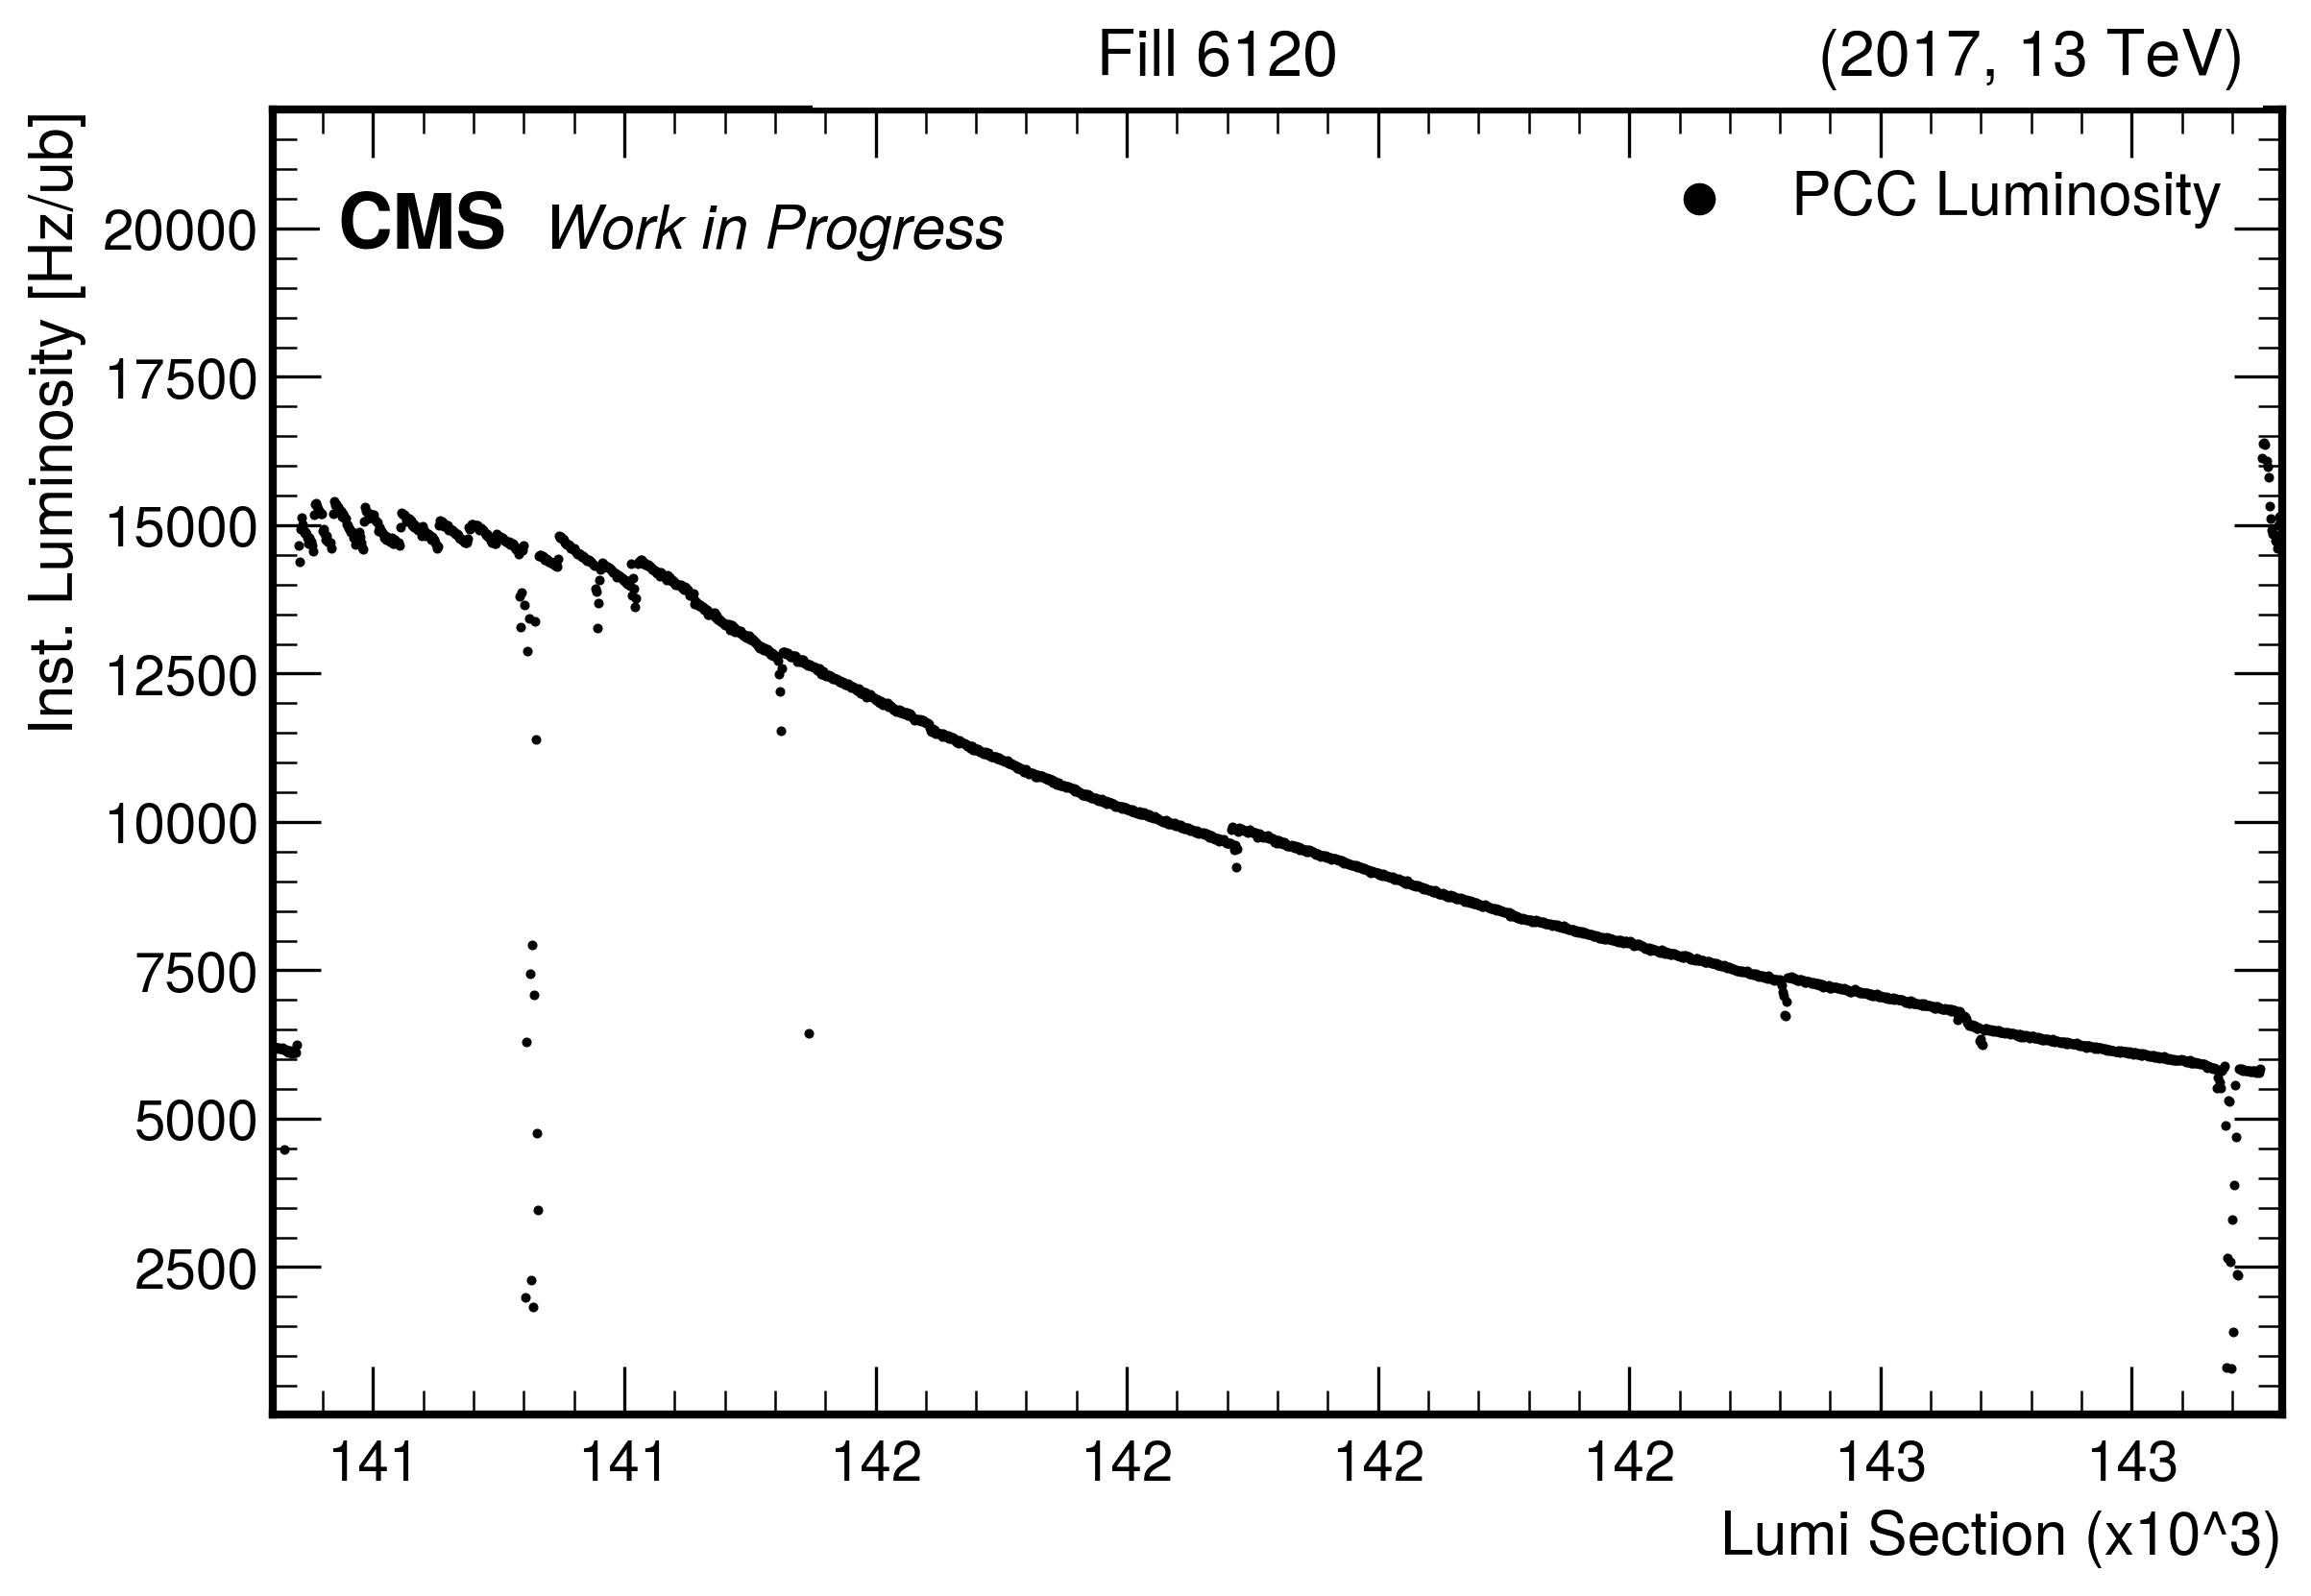
\includegraphics[width=.47\textwidth]{figures/performance_PCC/Lumi_2017_fill_6120.png}
    \caption[PCC Instantaneous Luminosity (Entire Year 2017) and Fill 7270 (2018)]{2017 PCC instantaneous luminosity as a function of lumi section for the entire year . (right) Instantaneous luminosity as measured offline as a function of time for LHC fill 7270 corresponding to the year 2018. The drops in luminosity correspond to emittance scans performed at the beginning and end of the fill, and to luminosity adjustments steps.}
    \label{Lumi_2017}
\end{figure}



The total CMS luminosity for 2017 and 2018 relies on multiple independently calibrated detectors: HFET, HFOC, PLT, and PCC. The final luminosity is obtained by averaging the measurements from these detectors. Ideally, all detectors would measure the same luminosity, making the average equivalent to any individual measurement. However, differences among the luminometers arise due to statistical fluctuations, applied rate corrections, the limited precision of the absolute calibrations and uncorrected instrumental effects.

Additional variations stem from time-dependent changes in detector performance and environmental conditions. These include factors such as detector aging, radiation damage, and noise fluctuations. In particular, detector aging can lead to gradual degradation in performance over time.

The stability systematic uncertainty is evaluated by assessing the consistency of each individual measurement with respect to the mean luminosity. This is done by computing the ratio of the luminosity measured by each independently calibrated luminometer (HFET, HFOC, PCC, and PLT) to the mean luminosity. Each ratio is averaged over time intervals of approximately 20 minutes (50 lumi sections), as shown in Fig.~\ref{fig:stabilitylinearity:stability}, where the upper row of the figure shows these ratios as a function of integrated luminosity, while the lower row displays their luminosity-weighted averages.

Finally, the standard deviation of the four averaged ratio values is taken as the stability uncertainty, amounting to \textbf{0.21\%} for 2017 and \textbf{0.30\%} for 2018.


\begin{figure}[!ht]
\centering
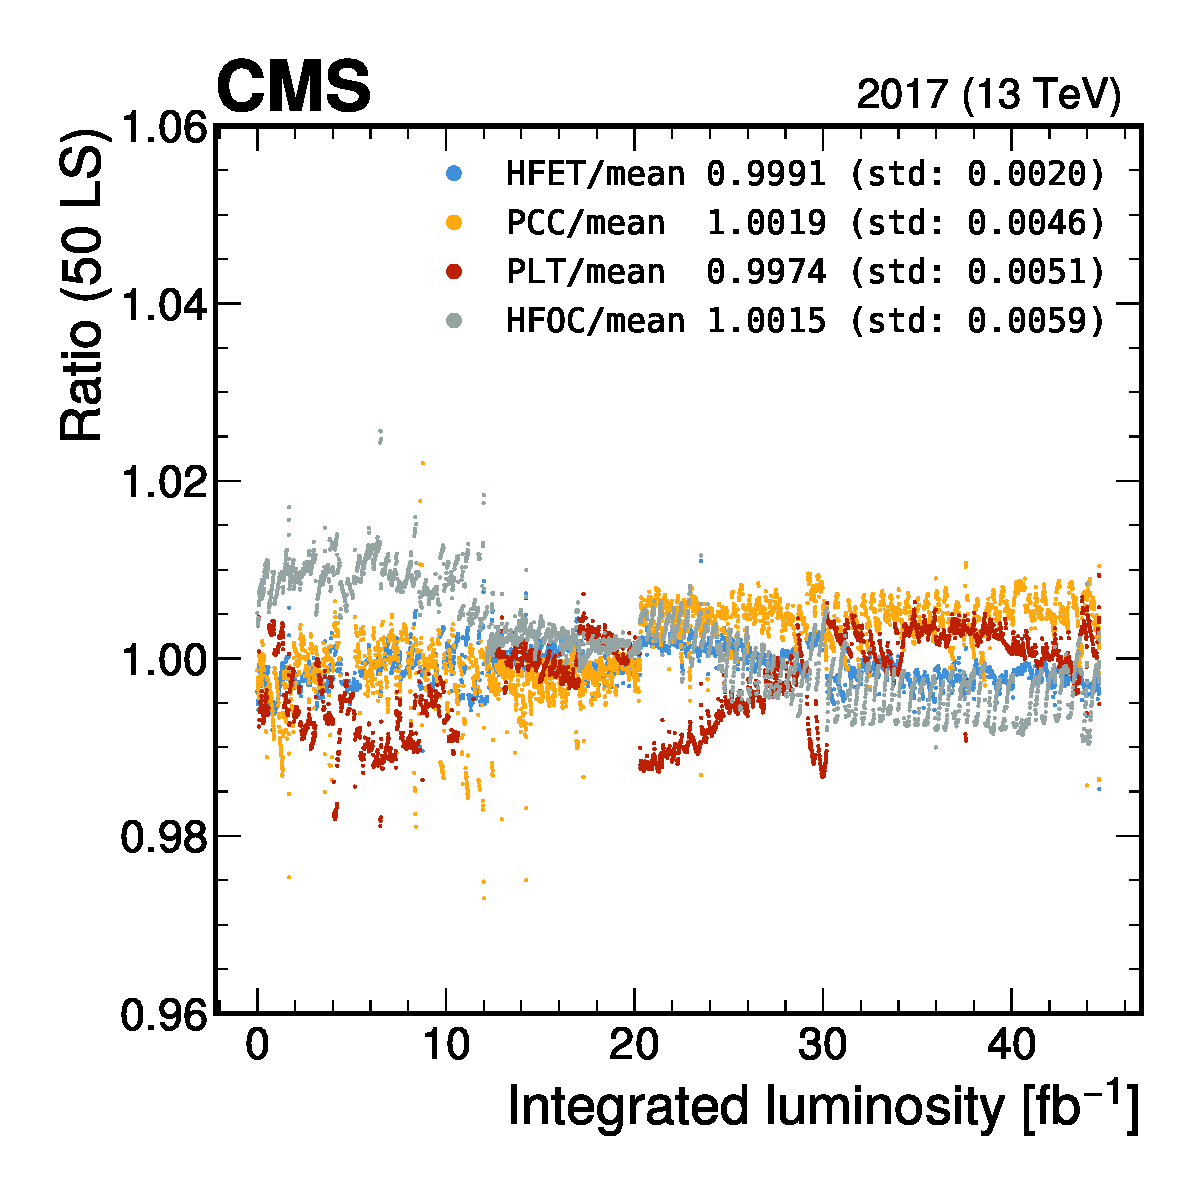
\includegraphics[width=0.45\textwidth]{figures/luminosity_integration_and_uncertainty/ratio__hfet-pcc-plt-hfocdivmean_PCConly_17.pdf}
\hspace*{0.05\textwidth}
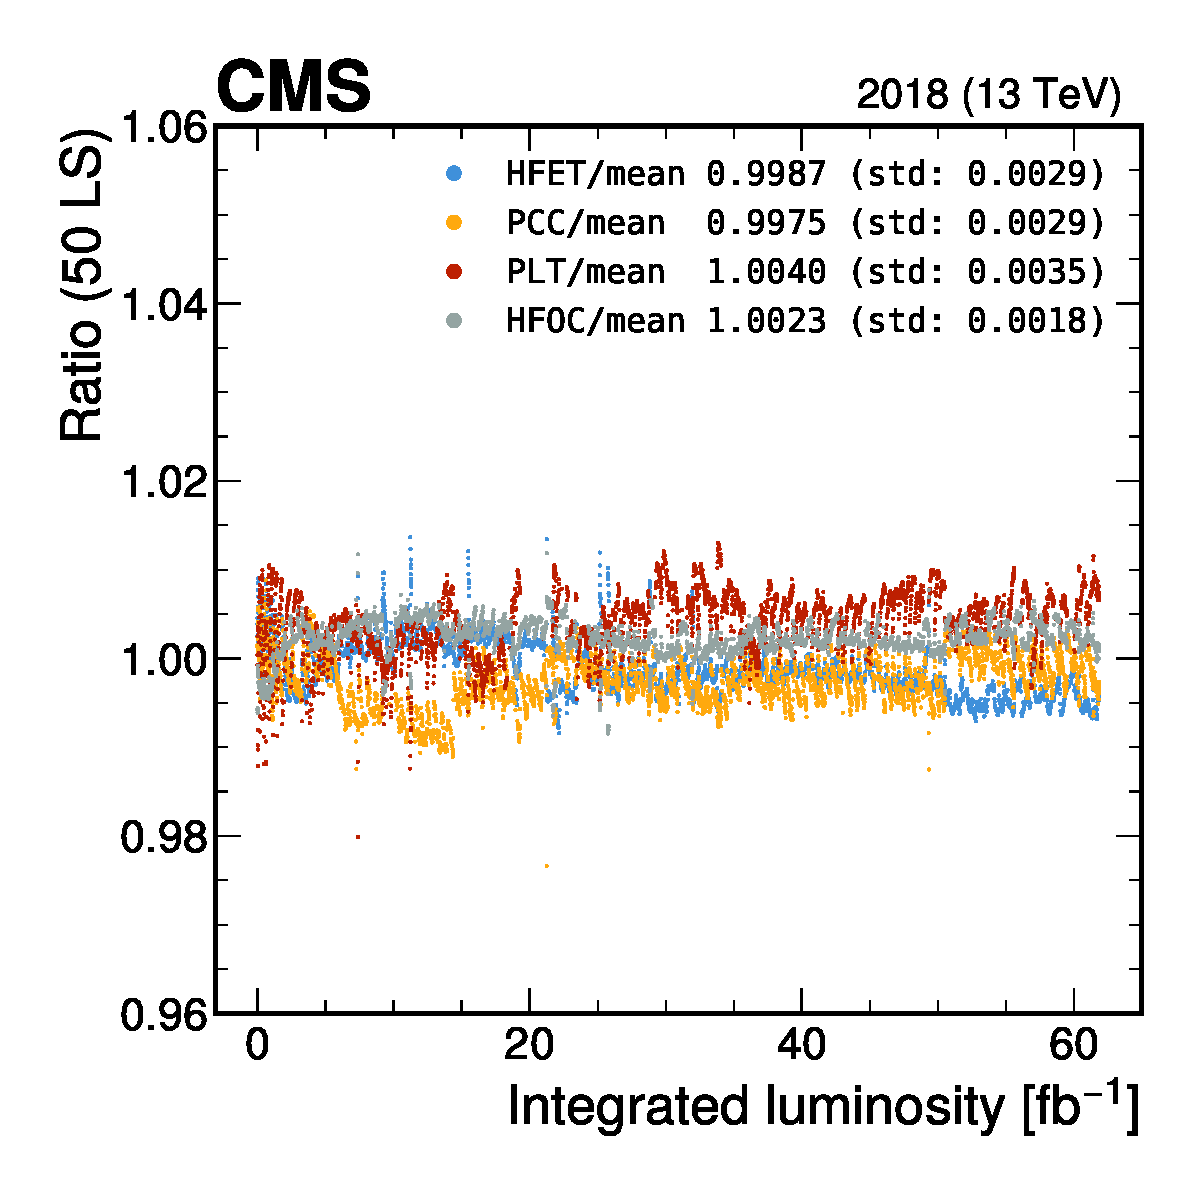
\includegraphics[width=0.45\textwidth]{figures/luminosity_integration_and_uncertainty/ratio__hfet-pcc-plt-hfocdivmean_PCConly_18.pdf}
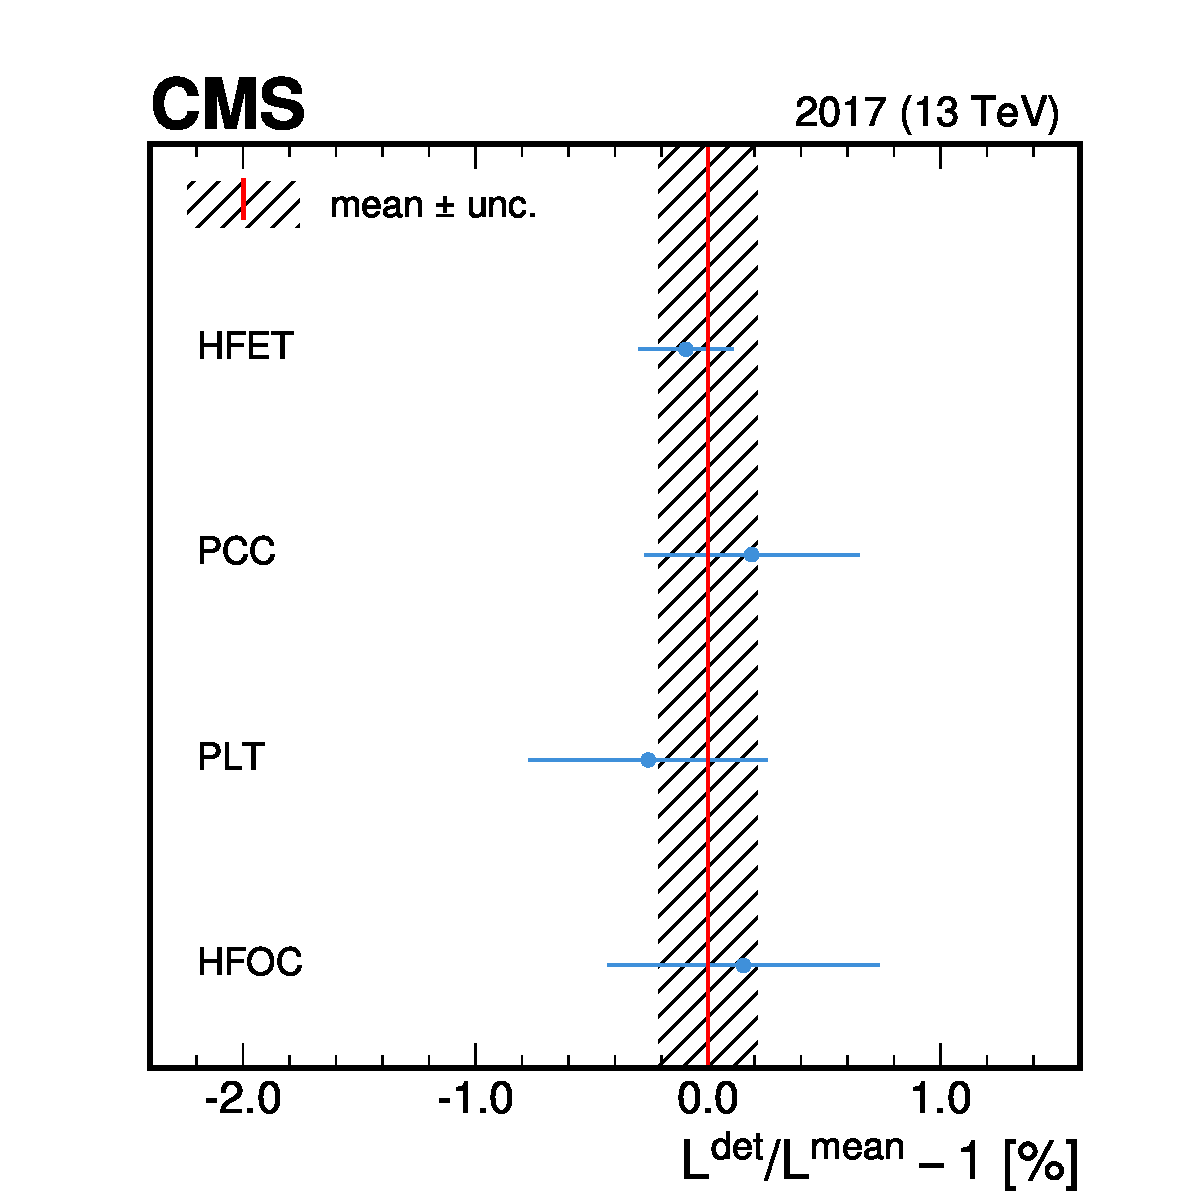
\includegraphics[width=0.45\textwidth]{figures/luminosity_integration_and_uncertainty/means_clean__hfet-pcc-plt-hfocdivmean_PCConly_17.pdf}
\hspace*{0.05\textwidth}
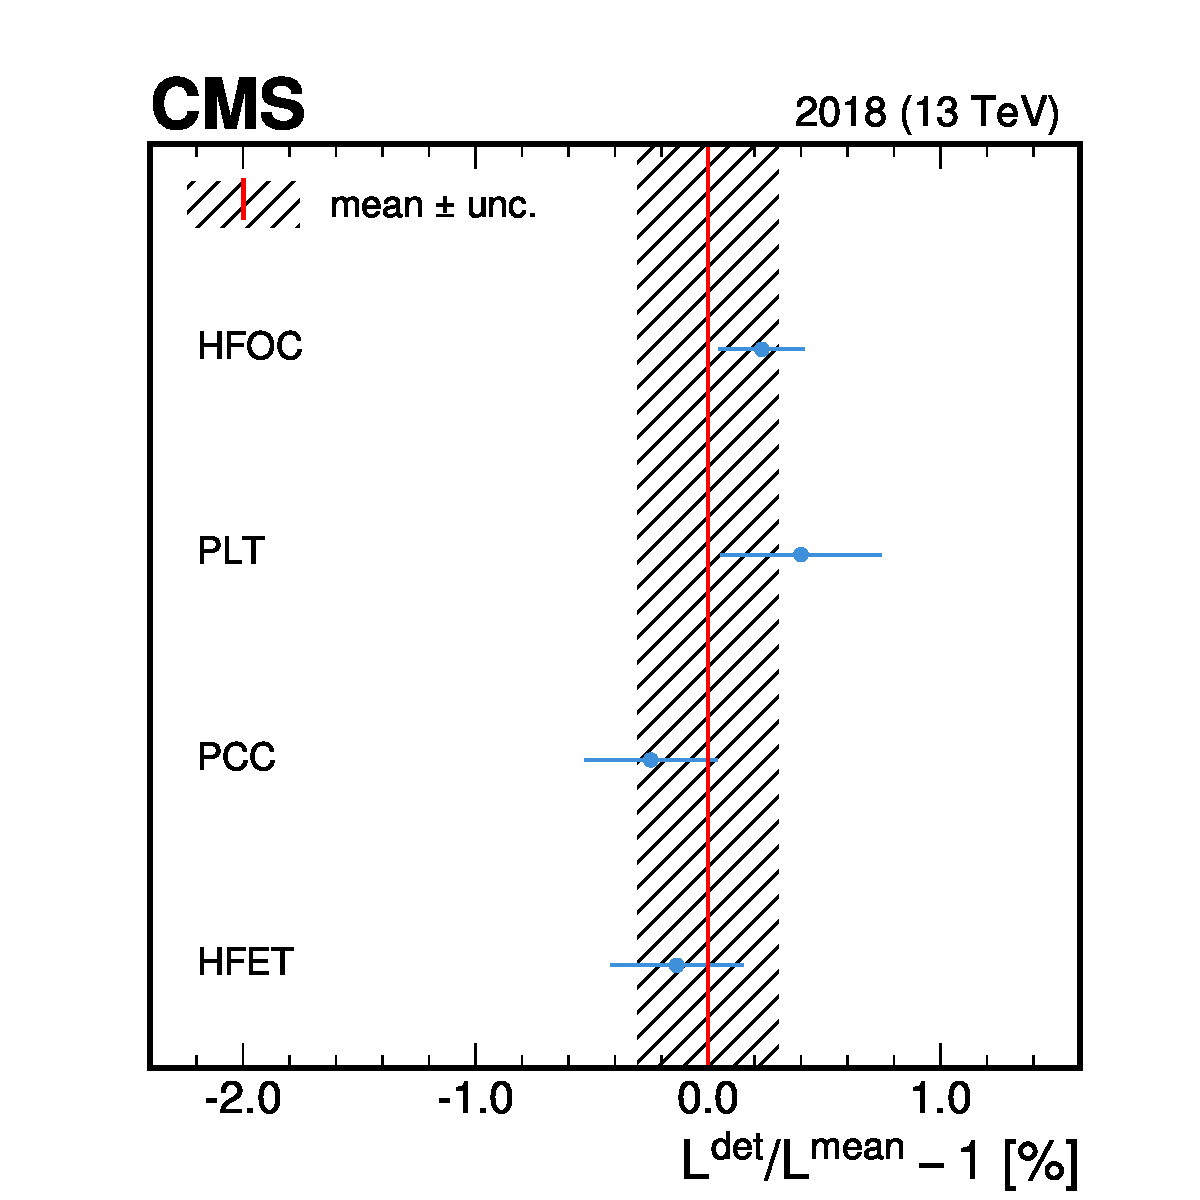
\includegraphics[width=0.45\textwidth]{figures/luminosity_integration_and_uncertainty/means_clean__hfet-pcc-plt-hfocdivmean_PCConly_18.pdf}
\caption[Luminosity Ratios (HFET, HFOC, PLT, PCC) to Mean per 50 LS Blocks (2017 & 2018)]{The ratio of the luminosity measured by HFET, HFOC, PLT and PCC to their mean per 50 LSblocks for 2017 (left) and 2018 (right). The upper row shows the ratio as a function of integrated luminosity, while the lower row displays the luminosity-weighted average of the ratios. The error bars signify the weighted standard deviation over the 20-minute units. The striped area represents the unweighted standard deviation of the four average ratio values.}
\label{fig:stabilitylinearity:stability}
\end{figure}

The linearity systematic uncertainty arises from the fact that a detector’s response may vary at different luminosity levels. This uncertainty is evaluated following the methodology described in previous publications~\cite{pas_17, pas_18}. The method consists of performing a linear fit to the ratio of the detector’s measured instantaneous luminosity to that of a reference luminometer, as a function of the reference single-bunch instantaneous luminosity (SBIL), taking advantage of the natural luminosity decay during each fill.

Only fills with a span of at least 2 Hz/$\mu$b and containing a minimum of five data points are considered. Each point represents an average over approximately six minutes (15 LS). Figure~\ref{fig:stabilitylinearity:linearity3}(right) shows an example of the linearity ratio for 2018 from fill 7272, comparing different detectors to the reference detector HFOC.

Due to their robust linear response, the final publication uses either DT or RAMSES~\cite{CMS:2021xjt} as the reference luminometer. The luminosity-weighted mean and standard deviation of the slopes obtained from comparisons with DT and RAMSES are shown in Figure~\ref{fig:stabilitylinearity:linearity3}. The larger of the two standard deviations is taken as the uncertainty estimate, yielding 0.081\%/(Hz/$\mu$b) for 2017 and 0.082\%/(Hz/$\mu$b) for 2018. The final linearity uncertainty on the integrated luminosity is computed by multiplying these values by the corresponding mean SBIL, resulting in uncertainties of 0.43\% for 2017 and 0.42\% for 2018.


\begin{figure}[!h]
\centering
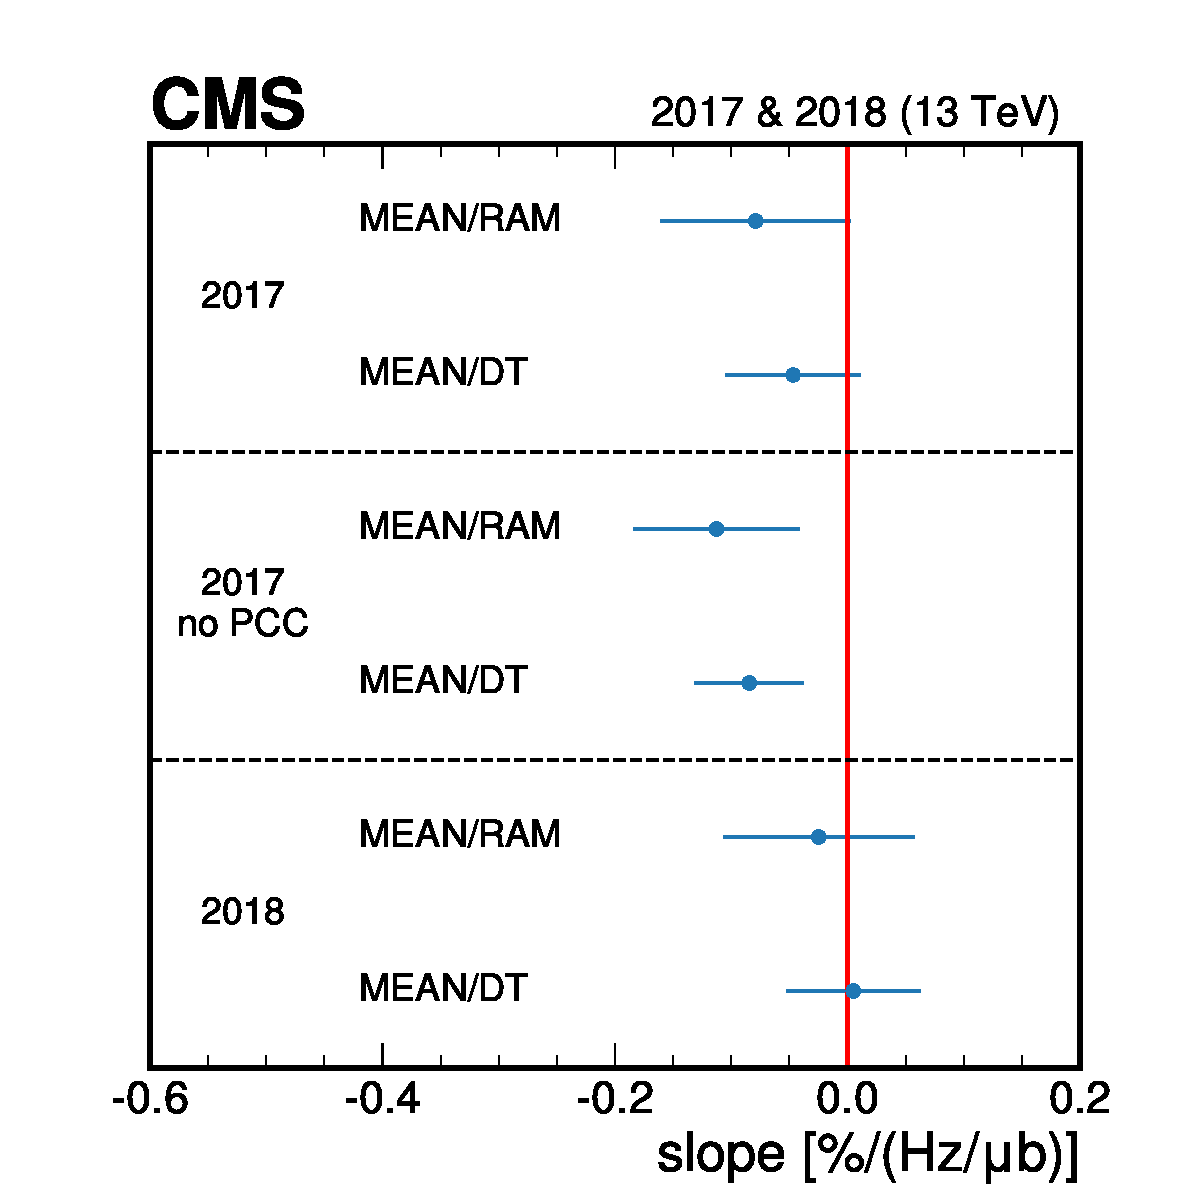
\includegraphics[width=0.45\textwidth]{figures/luminosity_integration_and_uncertainty/linearity_means_clean3.pdf}
\hspace*{0.05\textwidth}
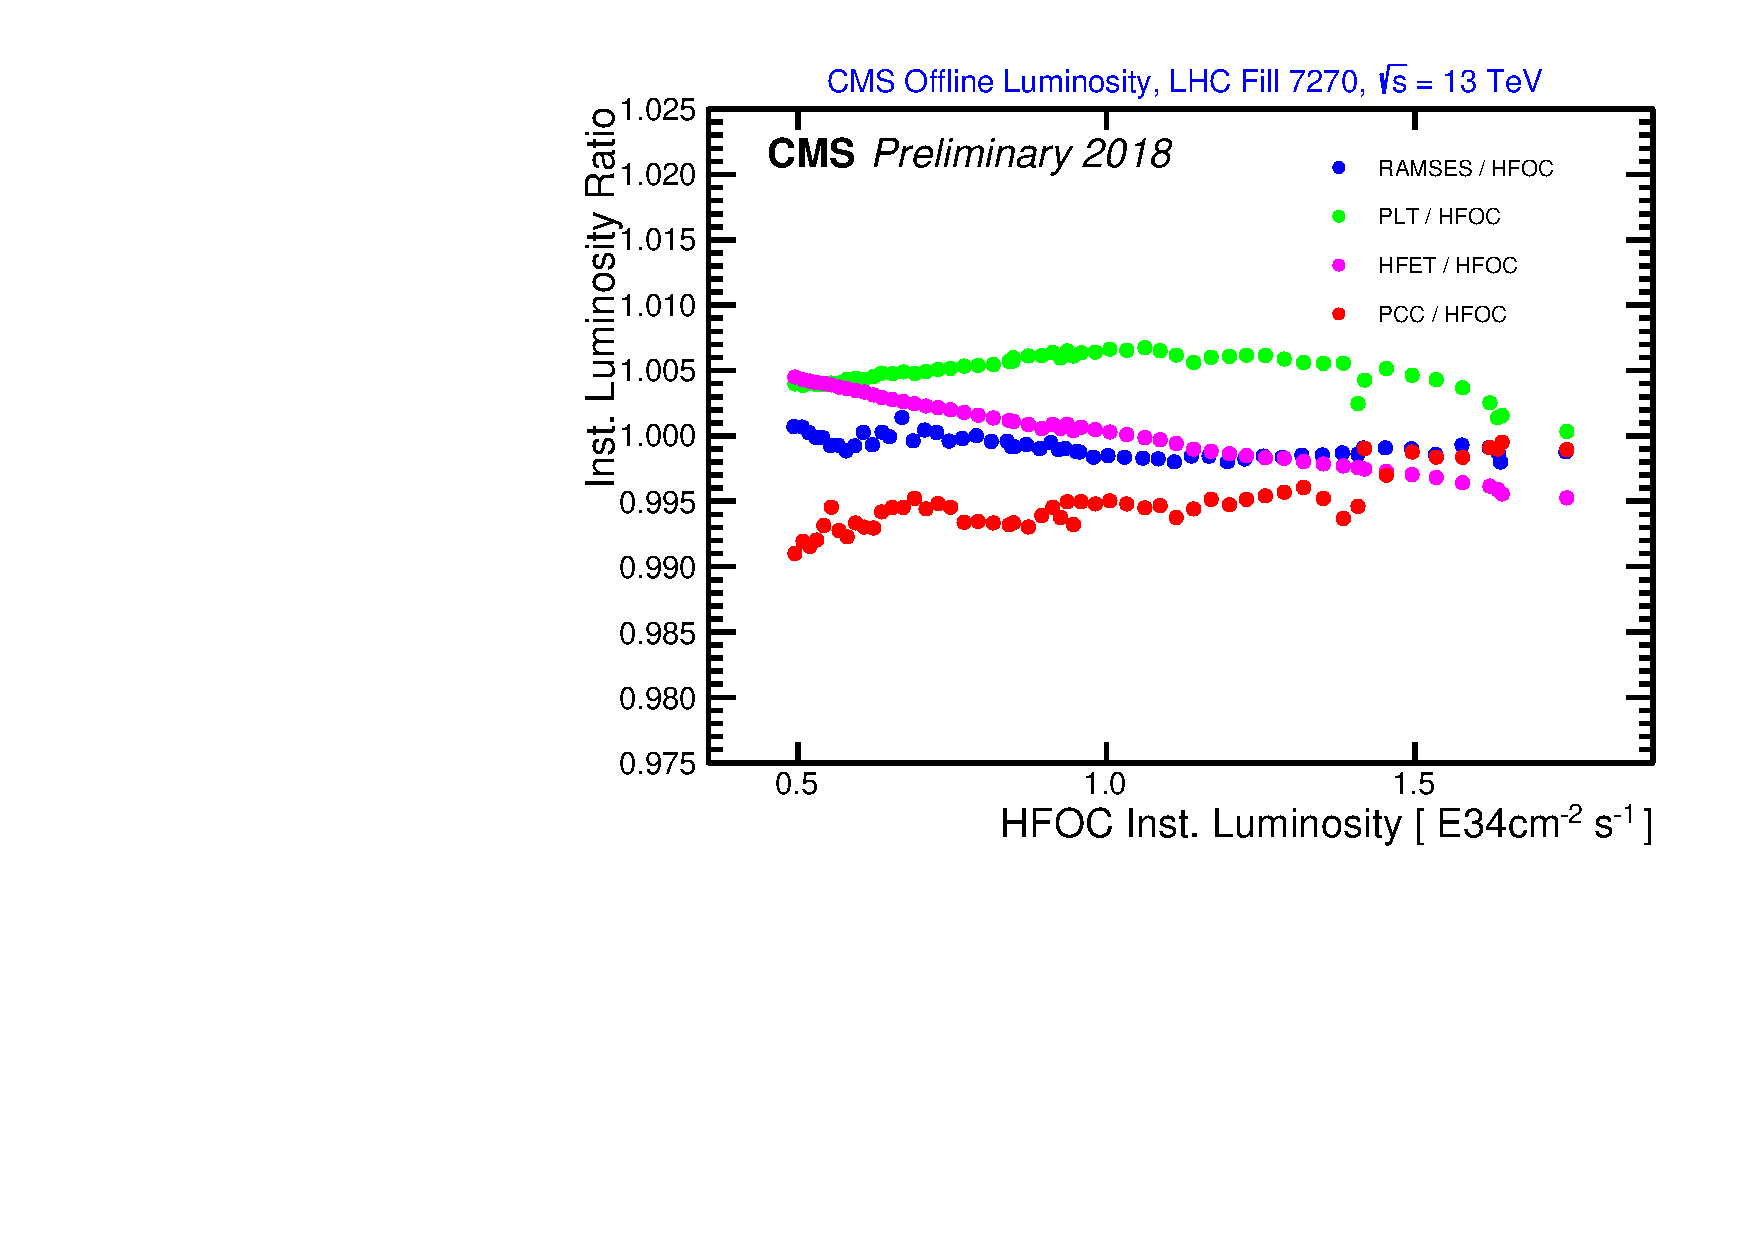
\includegraphics[width=0.45\textwidth]{figures/linearity_7270.pdf}
\caption[Residual Nonlinearity and Luminosity Ratios (2017 & 2018)]{(Right)The luminosity weighted average of the measured residual nonlinearity between the mean luminosity and DT or RAMSES (RAM) for 2017 and 2018. For 2017, the value is reported also for the mean without PCC, which is used for the low pile-up fills. The error bars signify the weighted standard deviation over the individual fills. (left)Ratios of instantaneous luminosity as measured offline by the CMS luminometers as a function of the instantaneous luminosity measured by HFOC for LHC fill 7270. The points correspond to intervals of 40 LS}
\label{fig:stabilitylinearity:linearity3}
\end{figure}






%The low pileup (low PU) data, recorded in a handful of fills in 2017, featuring an average SBIL of only 0.41 Hz/\(\mu\)b, are handled in an identical manner. In this region, PCC is not available for luminosity measurement due to poor statistical performance. 
%The sample standard deviation of the remaining three luminosity sources is 0.67\%, which is taken as the consistency uncertainty.

%The linearity uncertainty is estimated using the relative non-linearity slopes derived in high pileup conditions for the mean of HFOC, HFET and PLT with respect to DT and RAMSES. The value used (0.113\%(Hz/\(\mu\)b)$^{-1}$ 
%is the average relative slope between the three-detector mean and RAMSES. 
%Multiplied by the mean SBIL in the low pileup era, this results in a 0.04\% uncertainty. 


\section{Systematic Uncertainties}


The methods used to determine the integrated luminosity for the CMS proton-proton data collected in 2017 and 2018 at 13 TeV, as well as the sources of systematic uncertainty limiting its precision, have been discussed throughout this document. The final uncertainties are grouped into two main categories, normalization and integration. 


Normalization includes all uncertainties related to corrections applied during the final detector calibration with the determination of the visible cross section ($\sigma_{\text{vis}}$) using the vdM scan method, as described in Chapters~\ref{bbcorrections} and~\ref{Visible cross section results}. The dominant sources of uncertainty in this category are related to x-y factorizability, scan-to-scan variations, and cross-detector consistency during the vdM fills.

As discussed throughout the calibration corrections, the normalization uncertainties are considered correlated across years when they originate from the same underlying physical processes or instrumental sources, or when an identical methodology is the dominant contributor to the uncertainty. Exceptions include scan-to-scan and bunch-to-bunch variations in the measured $\sigma_{\text{vis}}$, as well as inconsistencies between the results from independent luminometers during the vdM fill. These factors are partly statistical or random in nature, and their underlying causes may vary from year to year.

The second actegory refers to the integration uncertainties, which relate to the efficiency and linearity of the detector response, as discussed in the previous chapter. These uncertainties arise from the stability and linearity of the different luminometers over the course of the entire year. In this case, cross-detector luminosity comparisons are treated as uncorrelated, whereas linearity uncertainties associated with the measured mean luminosity (calculated as the average of the values provided by the four bunch-by-bunch capable systems) are considered correlated.


Summing up the normalization and integration uncertainties, which contribute similarly to the total, the relative precision is 0.86\% in 2017 and 0.83\% in the high-pileup periods of 2018. Table \ref{TAB:SystematicError} provides a detailed summary of the uncertainties associated with the two main categories (normalization and integration) as well as the final consistency among the independently calibrated systems.

 

\begin{table}[H]
    %\centering
    \caption[Summary of the luminosity uncertainty components in 2017 and 2018]{Summary of the luminosity uncertainty components in 2017 and 2018, divided into normalization and integration categories.}
    \label{TAB:SystematicError}
    \begin{tabular}{|l|l|c|c|}
      \hline
      & Source                                        & 2017 [\%] & 2018 [\%] \\
      \hline\hline
      \multirow{10}{*}{Normalization} 
      & \hspace{+2mm} Ghost and satellite charge      & 0.06 & 0.07 \\
      & \hspace{+2mm} Beam current normalization      & 0.20 & 0.20 \\
      & \hspace{+2mm} Orbit drift                     & 0.09 & 0.19 \\
      & \hspace{+2mm} Beam-beam effects               & 0.29 & 0.30 \\
      & \hspace{+2mm} Length scale calibration        & 0.12 & 0.14 \\
      & \hspace{+2mm} Transverse factorizability      & 0.33 & 0.36 \\
      & \hspace{+2mm} Scan to scan variation          & 0.26 & 0.27 \\
      & \hspace{+2mm} Bunch to bunch variation        & 0.10 & 0.10 \\
      & \hspace{+2mm} Cross-detector consistency at vdM  & 0.41 & 0.14 \\
      \hline\hline
      \multirow{2}{*}{Integration} 
      & \hspace{+2mm} Cross-detector consistency per year & 0.21 & 0.30 \\
      & \hspace{+2mm} Linearity                       & 0.43 & 0.42 \\
      \hline\hline
      & \textbf{Total normalization uncertainty}      & \textbf{0.71} & \textbf{0.65} \\
      & \textbf{Total integration uncertainty}        & \textbf{0.48} & \textbf{0.52} \\
      & \textbf{Total uncertainty}                    & \textbf{0.86} & \textbf{0.83} \\
      \hline
    \end{tabular}
\end{table}
